% Generated by Sphinx.
\documentclass[letterpaper,12pt,spanish]{manual}
\usepackage[utf8]{inputenc}
\usepackage[T1]{fontenc}
\usepackage{babel}
\usepackage{times}
\usepackage[Sonny]{fncychap}
\usepackage{longtable}
\usepackage{sphinx}


\title{Manual del Desarrollador}
\date{June 20, 2011}
\release{1.0+0}
\author{Equipo de Desarrollo Canaima GNU/Linux}
\newcommand{\sphinxlogo}{}
\renewcommand{\releasename}{Release}
\makeindex
\makemodindex

\makeatletter
\def\PYG@reset{\let\PYG@it=\relax \let\PYG@bf=\relax%
    \let\PYG@ul=\relax \let\PYG@tc=\relax%
    \let\PYG@bc=\relax \let\PYG@ff=\relax}
\def\PYG@tok#1{\csname PYG@tok@#1\endcsname}
\def\PYG@toks#1+{\ifx\relax#1\empty\else%
    \PYG@tok{#1}\expandafter\PYG@toks\fi}
\def\PYG@do#1{\PYG@bc{\PYG@tc{\PYG@ul{%
    \PYG@it{\PYG@bf{\PYG@ff{#1}}}}}}}
\def\PYG#1#2{\PYG@reset\PYG@toks#1+\relax+\PYG@do{#2}}

\def\PYG@tok@gd{\def\PYG@tc##1{\textcolor[rgb]{0.63,0.00,0.00}{##1}}}
\def\PYG@tok@gu{\let\PYG@bf=\textbf\def\PYG@tc##1{\textcolor[rgb]{0.50,0.00,0.50}{##1}}}
\def\PYG@tok@gt{\def\PYG@tc##1{\textcolor[rgb]{0.00,0.25,0.82}{##1}}}
\def\PYG@tok@gs{\let\PYG@bf=\textbf}
\def\PYG@tok@gr{\def\PYG@tc##1{\textcolor[rgb]{1.00,0.00,0.00}{##1}}}
\def\PYG@tok@cm{\let\PYG@it=\textit\def\PYG@tc##1{\textcolor[rgb]{0.25,0.50,0.56}{##1}}}
\def\PYG@tok@vg{\def\PYG@tc##1{\textcolor[rgb]{0.73,0.38,0.84}{##1}}}
\def\PYG@tok@m{\def\PYG@tc##1{\textcolor[rgb]{0.13,0.50,0.31}{##1}}}
\def\PYG@tok@mh{\def\PYG@tc##1{\textcolor[rgb]{0.13,0.50,0.31}{##1}}}
\def\PYG@tok@cs{\def\PYG@tc##1{\textcolor[rgb]{0.25,0.50,0.56}{##1}}\def\PYG@bc##1{\colorbox[rgb]{1.00,0.94,0.94}{##1}}}
\def\PYG@tok@ge{\let\PYG@it=\textit}
\def\PYG@tok@vc{\def\PYG@tc##1{\textcolor[rgb]{0.73,0.38,0.84}{##1}}}
\def\PYG@tok@il{\def\PYG@tc##1{\textcolor[rgb]{0.13,0.50,0.31}{##1}}}
\def\PYG@tok@go{\def\PYG@tc##1{\textcolor[rgb]{0.19,0.19,0.19}{##1}}}
\def\PYG@tok@cp{\def\PYG@tc##1{\textcolor[rgb]{0.00,0.44,0.13}{##1}}}
\def\PYG@tok@gi{\def\PYG@tc##1{\textcolor[rgb]{0.00,0.63,0.00}{##1}}}
\def\PYG@tok@gh{\let\PYG@bf=\textbf\def\PYG@tc##1{\textcolor[rgb]{0.00,0.00,0.50}{##1}}}
\def\PYG@tok@ni{\let\PYG@bf=\textbf\def\PYG@tc##1{\textcolor[rgb]{0.84,0.33,0.22}{##1}}}
\def\PYG@tok@nl{\let\PYG@bf=\textbf\def\PYG@tc##1{\textcolor[rgb]{0.00,0.13,0.44}{##1}}}
\def\PYG@tok@nn{\let\PYG@bf=\textbf\def\PYG@tc##1{\textcolor[rgb]{0.05,0.52,0.71}{##1}}}
\def\PYG@tok@no{\def\PYG@tc##1{\textcolor[rgb]{0.38,0.68,0.84}{##1}}}
\def\PYG@tok@na{\def\PYG@tc##1{\textcolor[rgb]{0.25,0.44,0.63}{##1}}}
\def\PYG@tok@nb{\def\PYG@tc##1{\textcolor[rgb]{0.00,0.44,0.13}{##1}}}
\def\PYG@tok@nc{\let\PYG@bf=\textbf\def\PYG@tc##1{\textcolor[rgb]{0.05,0.52,0.71}{##1}}}
\def\PYG@tok@nd{\let\PYG@bf=\textbf\def\PYG@tc##1{\textcolor[rgb]{0.33,0.33,0.33}{##1}}}
\def\PYG@tok@ne{\def\PYG@tc##1{\textcolor[rgb]{0.00,0.44,0.13}{##1}}}
\def\PYG@tok@nf{\def\PYG@tc##1{\textcolor[rgb]{0.02,0.16,0.49}{##1}}}
\def\PYG@tok@si{\let\PYG@it=\textit\def\PYG@tc##1{\textcolor[rgb]{0.44,0.63,0.82}{##1}}}
\def\PYG@tok@s2{\def\PYG@tc##1{\textcolor[rgb]{0.25,0.44,0.63}{##1}}}
\def\PYG@tok@vi{\def\PYG@tc##1{\textcolor[rgb]{0.73,0.38,0.84}{##1}}}
\def\PYG@tok@nt{\let\PYG@bf=\textbf\def\PYG@tc##1{\textcolor[rgb]{0.02,0.16,0.45}{##1}}}
\def\PYG@tok@nv{\def\PYG@tc##1{\textcolor[rgb]{0.73,0.38,0.84}{##1}}}
\def\PYG@tok@s1{\def\PYG@tc##1{\textcolor[rgb]{0.25,0.44,0.63}{##1}}}
\def\PYG@tok@gp{\let\PYG@bf=\textbf\def\PYG@tc##1{\textcolor[rgb]{0.78,0.36,0.04}{##1}}}
\def\PYG@tok@sh{\def\PYG@tc##1{\textcolor[rgb]{0.25,0.44,0.63}{##1}}}
\def\PYG@tok@ow{\let\PYG@bf=\textbf\def\PYG@tc##1{\textcolor[rgb]{0.00,0.44,0.13}{##1}}}
\def\PYG@tok@sx{\def\PYG@tc##1{\textcolor[rgb]{0.78,0.36,0.04}{##1}}}
\def\PYG@tok@bp{\def\PYG@tc##1{\textcolor[rgb]{0.00,0.44,0.13}{##1}}}
\def\PYG@tok@c1{\let\PYG@it=\textit\def\PYG@tc##1{\textcolor[rgb]{0.25,0.50,0.56}{##1}}}
\def\PYG@tok@kc{\let\PYG@bf=\textbf\def\PYG@tc##1{\textcolor[rgb]{0.00,0.44,0.13}{##1}}}
\def\PYG@tok@c{\let\PYG@it=\textit\def\PYG@tc##1{\textcolor[rgb]{0.25,0.50,0.56}{##1}}}
\def\PYG@tok@mf{\def\PYG@tc##1{\textcolor[rgb]{0.13,0.50,0.31}{##1}}}
\def\PYG@tok@err{\def\PYG@bc##1{\fcolorbox[rgb]{1.00,0.00,0.00}{1,1,1}{##1}}}
\def\PYG@tok@kd{\let\PYG@bf=\textbf\def\PYG@tc##1{\textcolor[rgb]{0.00,0.44,0.13}{##1}}}
\def\PYG@tok@ss{\def\PYG@tc##1{\textcolor[rgb]{0.32,0.47,0.09}{##1}}}
\def\PYG@tok@sr{\def\PYG@tc##1{\textcolor[rgb]{0.14,0.33,0.53}{##1}}}
\def\PYG@tok@mo{\def\PYG@tc##1{\textcolor[rgb]{0.13,0.50,0.31}{##1}}}
\def\PYG@tok@mi{\def\PYG@tc##1{\textcolor[rgb]{0.13,0.50,0.31}{##1}}}
\def\PYG@tok@kn{\let\PYG@bf=\textbf\def\PYG@tc##1{\textcolor[rgb]{0.00,0.44,0.13}{##1}}}
\def\PYG@tok@o{\def\PYG@tc##1{\textcolor[rgb]{0.40,0.40,0.40}{##1}}}
\def\PYG@tok@kr{\let\PYG@bf=\textbf\def\PYG@tc##1{\textcolor[rgb]{0.00,0.44,0.13}{##1}}}
\def\PYG@tok@s{\def\PYG@tc##1{\textcolor[rgb]{0.25,0.44,0.63}{##1}}}
\def\PYG@tok@kp{\def\PYG@tc##1{\textcolor[rgb]{0.00,0.44,0.13}{##1}}}
\def\PYG@tok@w{\def\PYG@tc##1{\textcolor[rgb]{0.73,0.73,0.73}{##1}}}
\def\PYG@tok@kt{\def\PYG@tc##1{\textcolor[rgb]{0.56,0.13,0.00}{##1}}}
\def\PYG@tok@sc{\def\PYG@tc##1{\textcolor[rgb]{0.25,0.44,0.63}{##1}}}
\def\PYG@tok@sb{\def\PYG@tc##1{\textcolor[rgb]{0.25,0.44,0.63}{##1}}}
\def\PYG@tok@k{\let\PYG@bf=\textbf\def\PYG@tc##1{\textcolor[rgb]{0.00,0.44,0.13}{##1}}}
\def\PYG@tok@se{\let\PYG@bf=\textbf\def\PYG@tc##1{\textcolor[rgb]{0.25,0.44,0.63}{##1}}}
\def\PYG@tok@sd{\let\PYG@it=\textit\def\PYG@tc##1{\textcolor[rgb]{0.25,0.44,0.63}{##1}}}

\def\PYGZbs{\char`\\}
\def\PYGZus{\char`\_}
\def\PYGZob{\char`\{}
\def\PYGZcb{\char`\}}
\def\PYGZca{\char`\^}
% for compatibility with earlier versions
\def\PYGZat{@}
\def\PYGZlb{[}
\def\PYGZrb{]}
\makeatother

\begin{document}
\shorthandoff{"}
\maketitle
\tableofcontents
\hypertarget{--doc-index}{}


\textbf{Un conjunto de herramientas para la eliminación de las barreras tecnológicas}

Canaima Desarrollador (C-D) es un compendio de herramientas y ayudantes que facilitan el proceso de desarrollo de software para Canaima GNU/Linux. Está diseñado para \emph{facilitar el trabajo} a aquellas personas que participan en dicho proceso con regularidad, como también para \emph{iniciar a los que deseen aprender} de una manera rápida y práctica.

C-D sigue dos líneas de acción principales para lograr éste cometido: \emph{la práctica} y \emph{la formativa}. La práctica permite:
\begin{itemize}
\item {} 
Agilizar los procesos para la creación de paquetes binarios canaima a partir de paquetes fuentes correctamente estructurados.

\item {} 
Automatización personalizada de la creación de Paquetes Fuentes acordes a las Políticas de Canaima GNU/Linux.

\item {} 
Creación de un depósito personal, por usuario, donde se guardan automáticamente y en carpetas separadas los siguientes tipos de archivo:
- Proyectos en proceso de empaquetamiento
- Paquetes Binarios (\emph{.deb)
- Paquetes Fuente (}.tar.gz, \emph{.dsc, *.changes, *.diff)
- Registros provenientes de la creación de paquetes binarios (}.build)

\item {} 
Versionamiento asistido (basado en git) en los proyectos, brindando herramientas para realizar las siguientes operaciones, con un alto nivel de automatización y detección de posibles errores:
- git clone
- git commit
- git push
- git pull

\item {} 
Ejecución de tareas en masa (empaquetar, hacer pull, push, commit, entre otros), para agilizar procesos repetitivos.

\end{itemize}

En el otro aspecto, el formativo, C-D incluye:
\begin{itemize}
\item {} 
El Manual del Desarrollador, resumen técnico-práctico de las herramientas cognitivas necesarias para desarrollar paquetes funcionales para Canaima GNU/Linux.

\item {} 
La Guía de Referencia para el Desarrollador, compendio extenso y detallado que extiende y complementa el contenido del Manual del Desarrollador.

\item {} 
Éste manual para el uso de Canaima Desarrollador.

\end{itemize}


\bigskip\hrule{}\bigskip


\textbf{Índice de Contenidos}

\resetcurrentobjects
\hypertarget{--doc-man-canaima-desarrollador}{}

\chapter{\textbf{CANAIMA-DESARROLLADOR}}


\section{Un conjunto de herramientas para la eliminación de las barreras tecnológicas}
\begin{quote}\begin{description}
\item[{Author}] \leavevmode
Luis Alejandro Martínez Faneyth \textless{}\href{mailto:martinez.faneyth@gmail.com}{martinez.faneyth@gmail.com}\textgreater{}

\item[{Date}] \leavevmode
2011-01-22

\item[{Copyright}] \leavevmode
Libre uso, modificación y distribución (GPL3)

\item[{Version}] \leavevmode
1.0+0

\item[{Manual section}] \leavevmode
1

\item[{Manual group}] \leavevmode
Empaquetamiento

\end{description}\end{quote}


\subsection{\textbf{MODO DE USO}}

\begin{Verbatim}[commandchars=@\[\]]
canaima-desarrollador @PYGZlb[]AYUDANTE@PYGZrb[] @PYGZlb[]PARÁMETRO-1@PYGZrb[] @PYGZlb[]PARÁMETRO-2@PYGZrb[] ... @PYGZlb[]PARÁMETRO-N@PYGZrb[] @PYGZlb[]--ayuda@PYGZrb[]
\end{Verbatim}


\subsection{\textbf{DESCRIPCIÓN}}

Canaima Desarrollador (C-D) es un compendio de herramientas y ayudantes que facilitan el proceso de desarrollo de software para Canaima GNU/Linux. Está diseñado para \textbf{facilitar el trabajo} a aquellas personas que participan en dicho proceso con regularidad, como también para \textbf{iniciar a los que deseen aprender} de una manera rápida y práctica.

C-D puede ayudarte a:
\begin{itemize}
\item {} 
Agilizar los procesos para la creación de paquetes binarios canaima a partir de paquetes fuentes correctamente estructurados.

\item {} 
Automatización personalizada de la creación de Paquetes Fuentes acordes a las Políticas de Canaima GNU/Linux.

\item {} 
Creación de un depósito personal, por usuario, donde se guardan automáticamente y en carpetas separadas los siguientes tipos de archivo:
\begin{itemize}
\item {} 
Proyectos en proceso de empaquetamiento

\item {} 
Paquetes Binarios (*.deb)

\item {} 
Paquetes Fuente (*.tar.gz, *.dsc, *.changes, *.diff)

\item {} 
Registros provenientes de la creación de paquetes binarios (*.build)

\end{itemize}

\item {} 
Versionamiento asistido (basado en git) en los proyectos, brindando herramientas para realizar las siguientes operaciones, con un alto nivel de automatización y detección de posibles errores:
\begin{itemize}
\item {} 
git clone

\item {} 
git commit

\item {} 
git push

\item {} 
git pull

\end{itemize}

\item {} 
Ejecución de tareas en masa (empaquetar, hacer pull, push, commit, entre otros), para agilizar procesos repetitivos.

\end{itemize}


\subsection{\textbf{AYUDANTES DE CANAIMA DESARROLLADOR}}
\begin{itemize}
\item {} 
Crear Proyecto / Debianizar

\item {} 
Crear Fuente

\item {} 
Empaquetar

\item {} 
Descargar

\item {} 
Registrar

\item {} 
Enviar

\item {} 
Actualizar

\item {} 
Descargar Todo

\item {} 
Registrar Todo

\item {} 
Enviar Todo

\item {} 
Actualizar Todo

\item {} 
Empaquetar Varios

\item {} 
Empaquetar Todo

\item {} 
Listar Remotos

\item {} 
Listar Locales

\end{itemize}


\subsection{\textbf{CREAR PROYECTO / DEBIANIZAR}}

Crea un proyecto de empaquetamiento desde cero o debianiza uno existente.


\subsubsection{USO}

\begin{Verbatim}[commandchars=@\[\]]
canaima-desarrollador crear-proyecto@textbar[]debianizar --nombre="" --version="" --destino="" --licencia="" @PYGZlb[]--ayuda@PYGZrb[]
\end{Verbatim}


\subsubsection{PARÁMETROS}
\begin{description}
\item[{\code{-{-}nombre}}] \leavevmode
Un nombre para tu proyecto, que puede contener letras, números, puntos y guiones. Cualquier otro caracter no está permitido.

\item[{\code{-{-}version}}] \leavevmode
La versión inicial de tu proyecto. Se permiten números, guiones, puntos, letras o dashes (\textasciitilde{}).

\item[{\code{-{-}destino}}] \leavevmode
Especifica si es un proyecto de empaquetamiento para Canaima GNU/Linux o si es un proyecto personal. Las opciones disponibles son ``canaima'' y ``personal''.

\item[{\code{-{-}licencia}}] \leavevmode
Especifica el tipo de licencia bajo el cuál distribuirás tu trabajo. Las licencias soportadas son: apache, artistic, bsd, gpl, gpl2, gpl3, lgpl, lgpl2 y lgpl3.

\item[{\code{-{-}ayuda}}] \leavevmode
Muestra la documentación para el ayudante.

\end{description}

Si estás debianizando un proyecto existente, lo que ingreses en --nombre=''proyecto'' y --version=''X.Y+Z'' se utilizará para determinar cuál es el nombre de la carpeta a debianizar dentro del directorio del desarrollador, suponiendo que tiene el nombre proyecto-X.Y+Z. Si no se llama así, habrá un error.


\subsection{\textbf{CREAR FUENTE}}

Crea un paquete fuente a partir de un proyecto de empaquetamiento existente. El resultado es guardado en el depósito de fuentes.


\subsubsection{USO}

\begin{Verbatim}[commandchars=@\[\]]
canaima-desarrollador crear-fuente --directorio="" @PYGZlb[]--ayuda@PYGZrb[]
\end{Verbatim}


\subsubsection{PARÁMETROS}
\begin{description}
\item[{\code{-{-}directorio}}] \leavevmode
Nombre del directorio dentro de la carpeta del desarrollador donde se encuentra el proyecto. El directorio debe contener un proyecto debianizado.

\item[{\code{-{-}ayuda}}] \leavevmode
Muestra la documentación para el ayudante.

\end{description}


\subsection{\textbf{EMPAQUETAR}}

Éste ayudante te permite empaquetar un proyecto de forma automatizada, siguiendo la metodología git-buildpackage, que se centra en el siguiente diagrama:

\textbf{COMMIT \textgreater{} REFLEJAR CAMBIOS EN EL CHANGELOG \textgreater{} COMMIT \textgreater{} CREAR PAQUETE FUENTE \textgreater{} PUSH \textgreater{} GIT-BUILDPACKAGE}


\subsubsection{USO}

\begin{Verbatim}[commandchars=@\[\]]
canaima-desarrollador empaquetar --directorio="" --mensaje="" --procesadores="" @PYGZlb[]--ayuda@PYGZrb[]
\end{Verbatim}


\subsubsection{PARÁMETROS}
\begin{description}
\item[{\code{-{-}directorio}}] \leavevmode
Nombre de la carpeta dentro del directorio del desarrollador donde se encuentra el proyecto a empaquetar.

\item[{\code{-{-}mensaje}}] \leavevmode
Mensaje representativo de los cambios para el primer commit. El segundo commit es sólo para el changelog. Colocando la palabra ``auto'' o dejando el campo vacío, se autogenera el mensaje.

\item[{\code{-{-}procesadores}}] \leavevmode
Número de procesadores con que cuenta tu computadora para optimizar el proceso de empaquetamiento.

\item[{\code{-{-}ayuda}}] \leavevmode
Muestra la documentación para el ayudante.

\end{description}


\subsection{\textbf{DESCARGAR}}

Éste ayudante te permite copiar a tu disco duro un proyecto que se encuentre en el repositorio remoto para que puedas modificarlo según consideres. Utiliza git clone para realizar tal operación. Éste ayudante se encarga además de realizar las siguientes operaciones por ti:
\begin{itemize}
\item {} 
Verifica e informa sobre el éxito de la descarga.

\end{itemize}


\subsubsection{USO}

\begin{Verbatim}[commandchars=@\[\]]
canaima-desarrollador descargar --proyecto="" @PYGZlb[]--ayuda@PYGZrb[]
\end{Verbatim}


\subsubsection{PARÁMETROS}
\begin{description}
\item[{\code{-{-}proyecto}}] \leavevmode
Nombre del proyecto (en caso de que éste se encuentre en el repositorio de Canaima GNU/Linux) o la dirección git pública del proyecto.

\item[{\code{-{-}ayuda}}] \leavevmode
Muestra la documentación para el ayudante.

\end{description}


\subsection{\textbf{REGISTRAR}}

Éste ayudante te permite registar (o hacer commit de) los cambios hechos en un proyecto mediante el versionamiento basado en git. Utiliza git commit para lograr éste propósito. Éste ayudante se encarga además de realizar las siguientes operaciones por ti:
\begin{itemize}
\item {} 
Verifica la existencia de la rama git ``upstream''. En caso de no encontrarla, la crea.

\item {} 
Verifica la existencia de la rama git ``master''. En caso de no encontrarla, la crea.

\item {} 
Verifica la existencia de todos los elementos necesarios para ejecutar la acción git commit (carpetas, variables de entorno, etc..). En caso de encontrar algún error, aborta e informa.

\item {} 
Autogenera el mensaje de commit, si se le instruye.

\item {} 
Hace git checkout a la rama master, si nos encontramos en una rama diferente a la hora de hace commit.

\item {} 
Hace un git merge de la rama master a la upstream, inmediatamente depués del commit.

\end{itemize}


\subsubsection{USO}

\begin{Verbatim}[commandchars=@\[\]]
canaima-desarrollador registrar --directorio="" --mensaje=="" @PYGZlb[]--ayuda@PYGZrb[]
\end{Verbatim}


\subsubsection{PARÁMETROS}
\begin{description}
\item[{\code{-{-}directorio}}] \leavevmode
Nombre de la carpeta dentro del directorio del desarrollador a la que se quiere hacer commit.

\item[{\code{-{-}mensaje}}] \leavevmode
Mensaje representativo de los cambios para el commit. Colocando la palabra ``auto'' o dejando el campo vacío, se autogenera el mensaje.

\item[{\code{-{-}ayuda}}] \leavevmode
Muestra la documentación para el ayudante.

\end{description}


\subsection{\textbf{ENVIAR}}

Éste ayudante te permite enviar los cambios realizados al repositorio remoto especificado en las configuraciones personales, mediante el uso de la acción git push. Éste ayudante se encarga además de realizar las siguientes operaciones por ti:
\begin{itemize}
\item {} 
Verifica la existencia de la rama git ``upstream''. En caso de no encontrarla, la crea.

\item {} 
Verifica la existencia de la rama git ``master''. En caso de no encontrarla, la crea.

\item {} 
Verifica la existencia de todos los elementos necesarios para ejecutar la acción git push (carpetas, variables de entorno, etc..). En caso de encontrar algún error, aborta e informa.

\item {} 
Configura el repositorio remoto para el proyecto, de acuerdo a los parámetros establecidos en \textasciitilde{}/.config/canaima-desarrollador/usuario.conf

\end{itemize}


\subsubsection{USO}

\begin{Verbatim}[commandchars=@\[\]]
canaima-desarrollador enviar --directorio="" @PYGZlb[]--ayuda@PYGZrb[]
\end{Verbatim}


\subsubsection{PARÁMETROS}
\begin{description}
\item[{\code{-{-}directorio}}] \leavevmode
Nombre de la carpeta dentro del directorio del desarrollador a la que se quiere hacer push.

\item[{\code{-{-}ayuda}}] \leavevmode
Muestra la documentación para el ayudante.

\end{description}


\subsection{\textbf{ACTUALIZAR}}

Éste ayudante te permite actualizar el código fuente de un determinado proyecto, mediante la ejecución de ``git pull'' en la carpeta del proyecto. Éste ayudante se encarga además de realizar las siguientes operaciones por ti:
\begin{itemize}
\item {} 
Verifica la existencia de la rama git ``upstream''. En caso de no encontrarla, la crea.

\item {} 
Verifica la existencia de la rama git ``master''. En caso de no encontrarla, la crea.

\item {} 
Verifica la existencia de todos los elementos necesarios para ejecutar la acción git pull (carpetas, variables de entorno, etc..). En caso de encontrar algún error, aborta e informa.

\item {} 
Configura el repositorio remoto para el proyecto, de acuerdo a los parámetros establecidos en \textasciitilde{}/.config/canaima-desarrollador/usuario.conf

\end{itemize}


\subsubsection{USO}

\begin{Verbatim}[commandchars=@\[\]]
canaima-desarrollador actualizar --directorio="" @PYGZlb[]--ayuda@PYGZrb[]
\end{Verbatim}


\subsubsection{PARÁMETROS}
\begin{description}
\item[{\code{-{-}directorio}}] \leavevmode
Nombre de la carpeta dentro del directorio del desarrollador a la que se quiere hacer git pull.

\item[{\code{-{-}ayuda}}] \leavevmode
Muestra la documentación para el ayudante.

\end{description}


\subsection{\textbf{DESCARGAR TODO}}

Éste ayudante te permite copiar a tu disco duro todos los proyectos de Canaima GNU/Linux que se encuentren en el repositorio remoto oficial. Utiliza git clone para realizar tal operación.


\subsubsection{USO}

\begin{Verbatim}[commandchars=@\[\]]
canaima-desarrollador descargar-todo @PYGZlb[]--ayuda@PYGZrb[]
\end{Verbatim}


\subsubsection{PARÁMETROS}
\begin{description}
\item[{\code{-{-}ayuda}}] \leavevmode
Muestra la documentación para el ayudante.

\end{description}


\subsection{\textbf{REGISTRAR TODO}}

Éste ayudante te permite registar (o hacer commit de) todos los cambios hechos en todos los proyectos existentes en la carpeta del desarrollador. Utiliza git commit para lograr éste propósito. Asume un mensaje de commit automático para todos.


\subsubsection{USO}

\begin{Verbatim}[commandchars=@\[\]]
canaima-desarrollador registrar-todo @PYGZlb[]--ayuda@PYGZrb[]
\end{Verbatim}


\subsubsection{PARÁMETROS}
\begin{description}
\item[{\code{-{-}ayuda}}] \leavevmode
Muestra la documentación para el ayudante.

\end{description}


\subsection{\textbf{ENVIAR TODO}}

Éste ayudante te permite enviar todos los cambios realizados en todos los proyectos ubicados en la carpeta del desarrollador al repositorio remoto especificado en las configuraciones personales, mediante el uso de la acción git push.


\subsubsection{USO}

\begin{Verbatim}[commandchars=@\[\]]
canaima-desarrollador enviar-todo @PYGZlb[]--ayuda@PYGZrb[]
\end{Verbatim}


\subsubsection{PARÁMETROS}
\begin{description}
\item[{\code{-{-}ayuda}}] \leavevmode
Muestra la documentación para el ayudante.

\end{description}


\subsection{\textbf{ACTUALIZAR TODO}}

Éste ayudante te permite actualizar el código fuente de todos los proyectos ubicados en la carpeta del desarrollador, mediante la ejecución de ``git pull'' en la carpeta del proyecto.


\subsubsection{USO}

\begin{Verbatim}[commandchars=@\[\]]
canaima-desarrollador actualizar-todo @PYGZlb[]--ayuda@PYGZrb[]
\end{Verbatim}


\subsubsection{PARÁMETROS}
\begin{description}
\item[{\code{-{-}ayuda}}] \leavevmode
Muestra la documentación para el ayudante.

\end{description}


\subsection{\textbf{EMPAQUETAR VARIOS}}

Éste ayudante te permite empaquetar varios proyectos.


\subsubsection{USO}

\begin{Verbatim}[commandchars=@\[\]]
canaima-desarrollador empaquetar-varios --para-empaquetar="" --procesadores="" @PYGZlb[]--ayuda@PYGZrb[]
\end{Verbatim}


\subsubsection{PARÁMETROS}
\begin{description}
\item[{\code{-{-}para-empaquetar}}] \leavevmode
Lista de los directorios dentro de la carpeta del desarrollador que contienen los proyectos que se quieren empaquetar, agrupados entre comillas.

\item[{\code{-{-}procesadores}}] \leavevmode
Número de procesadores con que cuenta tu computadora para optimizar el proceso de empaquetamiento.

\item[{\code{-{-}ayuda}}] \leavevmode
Muestra la documentación para el ayudante.

\end{description}


\subsection{\textbf{EMPAQUETAR TODO}}

Éste ayudante te permite empaquetar todos los proyectos existentes en la carpeta del desarrollador.


\subsubsection{USO}

\begin{Verbatim}[commandchars=@\[\]]
canaima-desarrollador empaquetar-todo --procesadores="" @PYGZlb[]--ayuda@PYGZrb[]
\end{Verbatim}


\subsubsection{PARÁMETROS}
\begin{description}
\item[{\code{-{-}procesadores}}] \leavevmode
Número de procesadores con que cuenta tu computadora para optimizar el proceso de empaquetamiento.

\item[{\code{-{-}ayuda}}] \leavevmode
Muestra la documentación para el ayudante.

\end{description}


\subsection{\textbf{LISTAR REMOTOS}}

Muestra todos los proyectos contenidos en el repositorio remoto y muestra su dirección git.


\subsubsection{USO}

\begin{Verbatim}[commandchars=@\[\]]
canaima-desarrollador listar-remotos @PYGZlb[]--ayuda@PYGZrb[]
\end{Verbatim}


\subsubsection{PARÁMETROS}
\begin{description}
\item[{\code{-{-}ayuda}}] \leavevmode
Muestra la documentación para el ayudante.

\end{description}


\subsection{\textbf{LISTAR LOCALES}}

Muestra todos los proyectos contenidos en la carpeta del desarrollador y los clasifica según su tipo.


\subsubsection{USO}

\begin{Verbatim}[commandchars=@\[\]]
canaima-desarrollador listar-locales @PYGZlb[]--ayuda@PYGZrb[]
\end{Verbatim}


\subsubsection{PARÁMETROS}
\begin{description}
\item[{\code{-{-}ayuda}}] \leavevmode
Muestra la documentación para el ayudante.

\end{description}

\resetcurrentobjects
\hypertarget{--doc-manual-desarrollador}{}

\chapter{\textbf{Manual para el Desarrollador}}

Es bien sabido que Canaima GNU/Linux es una de las distribuciones de Software Libre más importantes de Venezuela. Actualmente se incluye en más de 880 mil portátiles del proyecto Canaima Educativo, ha sido descargado más de 120 mil veces del portal oficial y se planea extender el Proyecto a toda la Administración Pública Nacional.

Sin embargo, la popularidad no lo es todo. Detrás de Canaima GNU/Linux existe un ciclo de desarrollo bastante particular, propio de la dinámica socio-tecnológica en que está envuelto. Éste documento describirá la metodología mediante la cual el colectivo asociado a la Metadistribución, participa en los procesos socio-productivos y de desarrollo que impulsan la generación de Nuevas versiones de Canaima y sustentan su plataforma tecnológica.


\section{\textbf{Sobre el Ciclo de Desarrollo de Canaima}}

Podemos decir que básicamente el ciclo de desarrollo de Canaima sigue un flujo natural de los acontecimientos tal cual se reseñan en el esquema inferior.

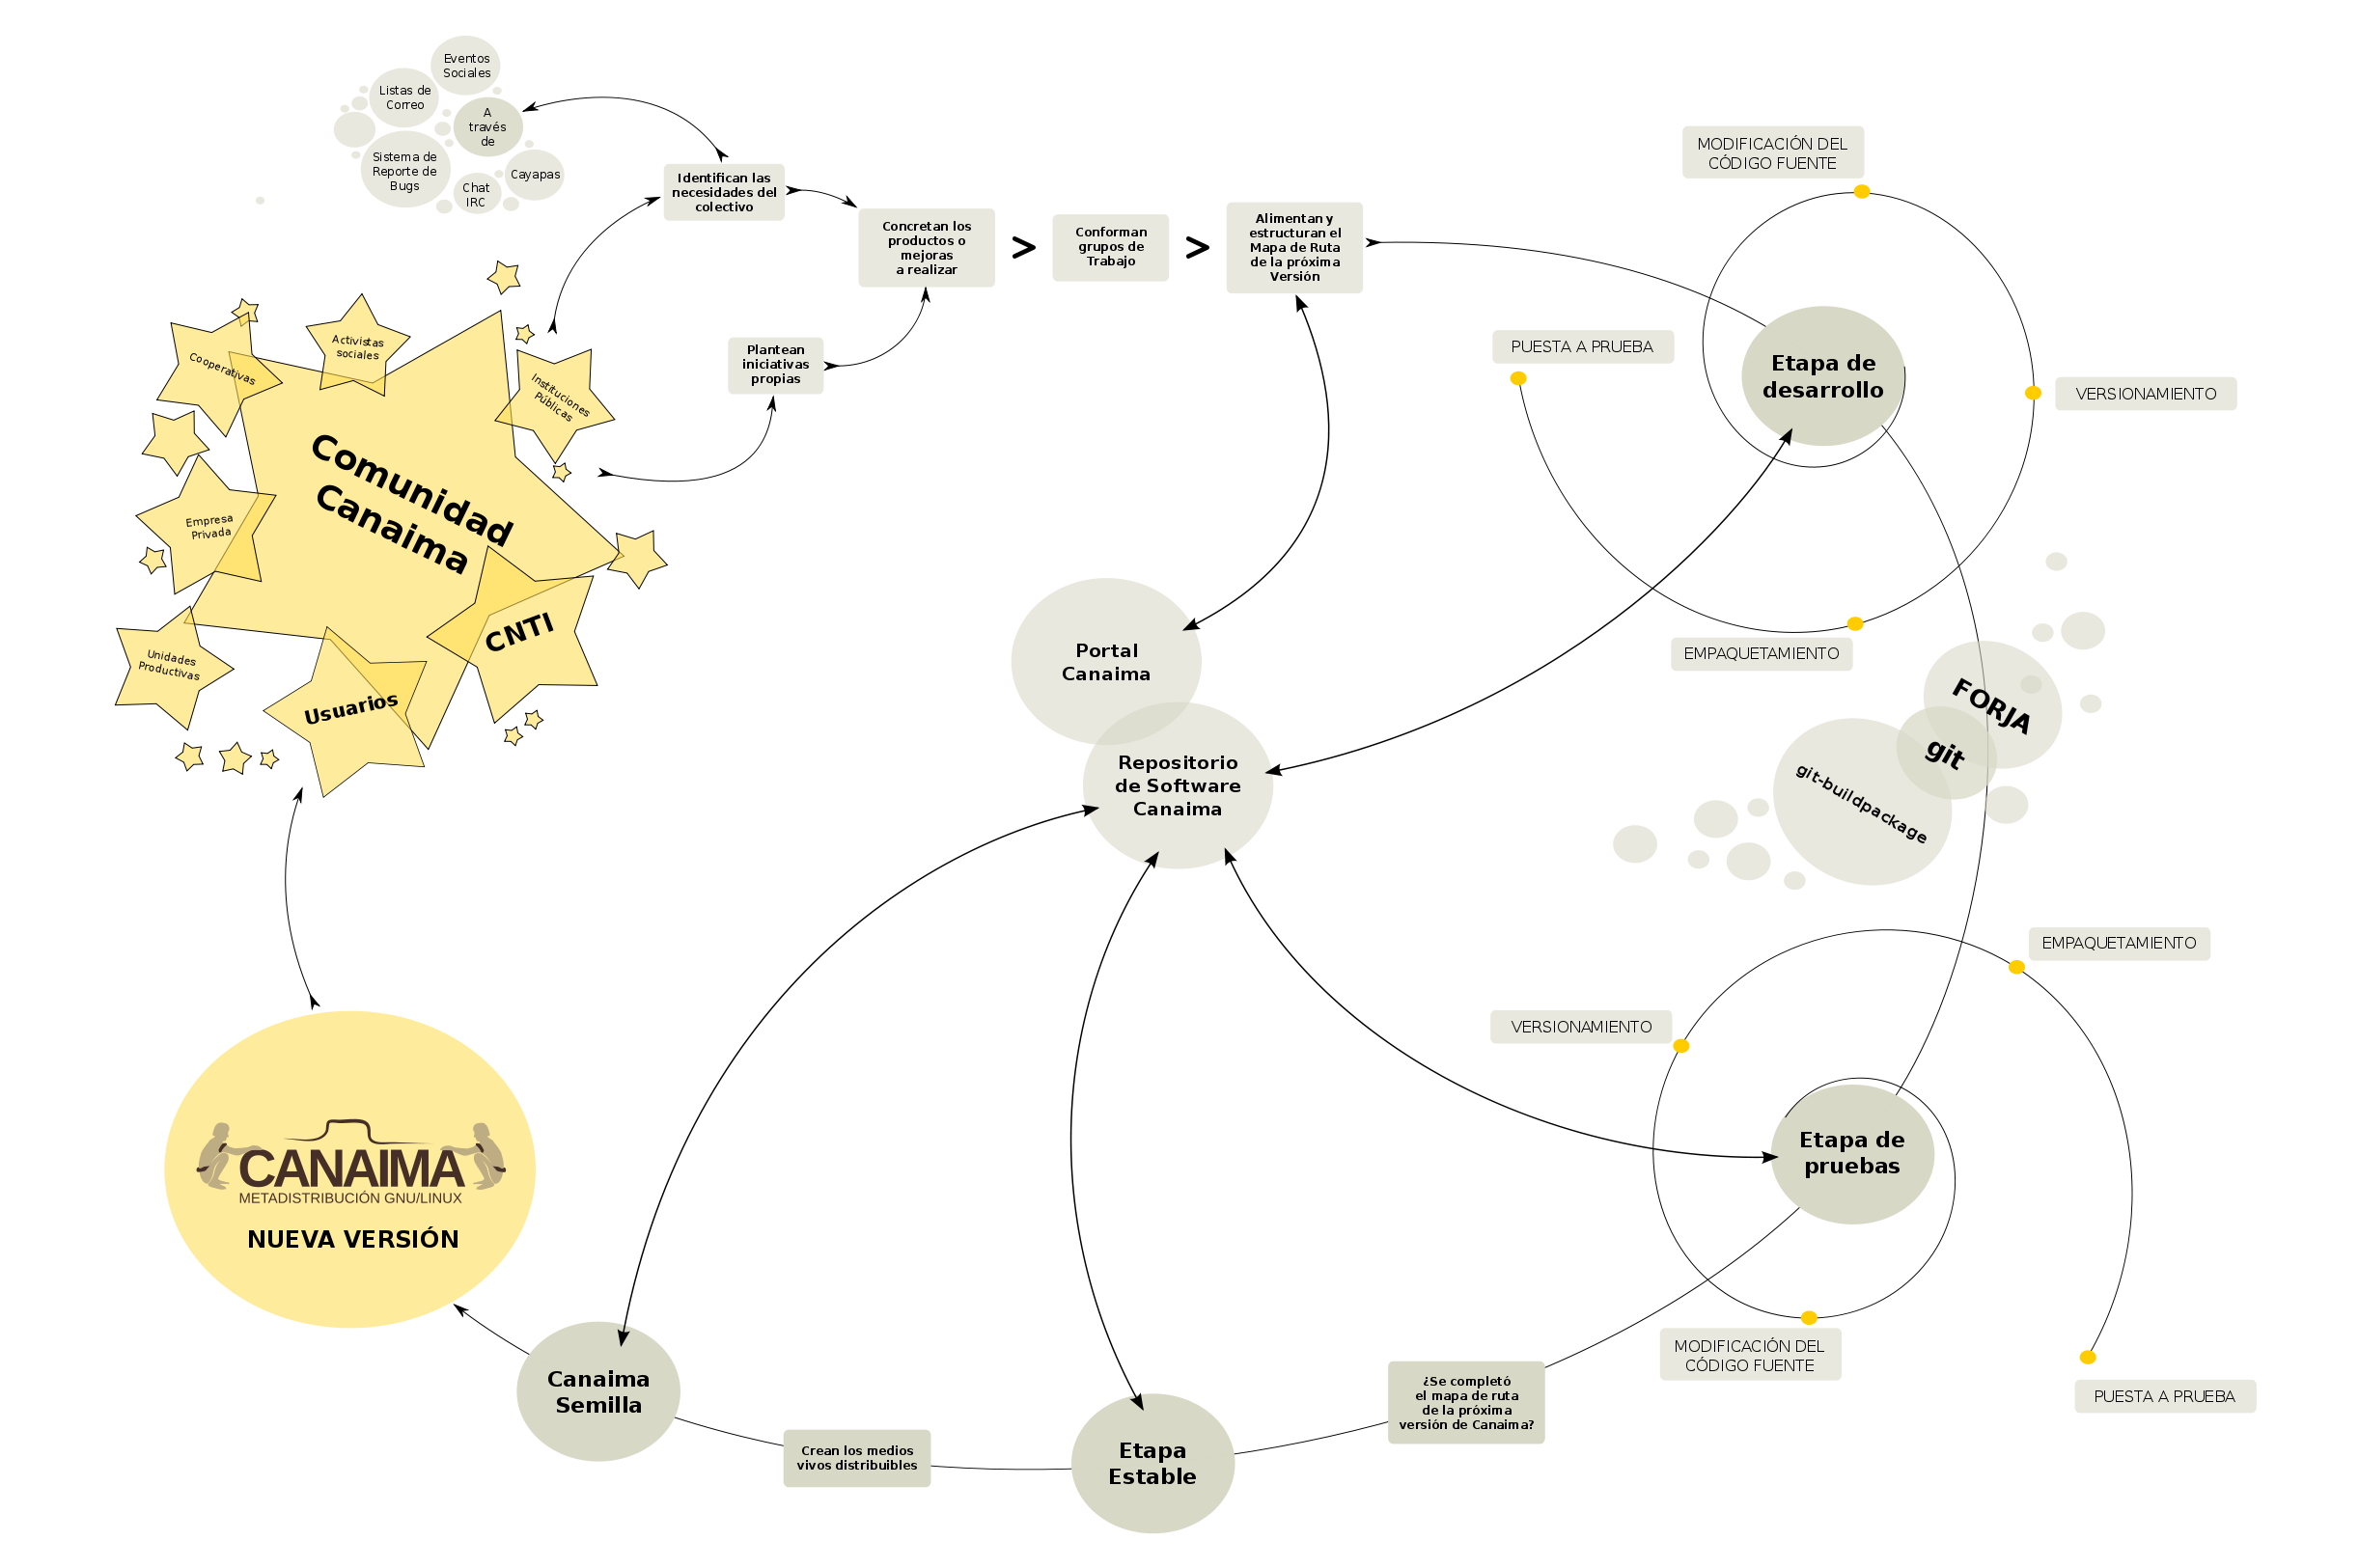
\includegraphics{diagrama.png}


\subsection{¿Quienes son los actores?}

La comunidad canaima está conformada por un gran número de personas que tienen intereses comunes y que comparten un mismo espacio virtual conformado por una serie de herramientas y servicios condensados en una plataforma pública. Éstos actores provienen de distintas organizaciones y colectivos, a saber: el \href{http://www.cnti.gob.ve/}{CNTI}, Instituciones Públicas en general, Unidades Productivas, Cooperativas, Empresas Privadas, Activistas Sociales y Usuarios en general.

Éste conjunto de personas poseen una dinámica propia, característica de sus realidades particulares; sin embargo, es posible diferenciar un ciclo que se ejecuta cada vez que se publica una nueva versión de Canaima GNU/Linux.


\subsection{Cocinando una nueva versión de Canaima GNU/Linux}

En teoría, una versión de Canaima es publicada cada \textasciitilde{}6 meses en sincronía con la \href{http://cayapa.canaima.softwarelibre.gob.ve/}{Cayapa}. Para que ésto se cumpla, ciertos hitos deben ser alcanzados.

\textbf{La primera meta es realizar un producto}. ¿Quien puede realizar un producto para Canaima GNU/Linux? Cualquiera puede hacerlo, sin embargo te recomendamos ciertas cosas que te ayudarán a hacerlo con mayor calidad y eficiencia:
\begin{itemize}
\item {} 
Aprende a empaquetar con git-buildpackage (más abajo).

\item {} 
Participa en la lista de correo \href{http://listas.canaima.softwarelibre.gob.ve/cgi-bin/mailman/listinfo/desarrolladores}{desarrolladores}, \href{http://listas.canaima.softwarelibre.gob.ve/cgi-bin/mailman/listinfo/discusion}{discusion} y \href{http://listas.canaima.softwarelibre.gob.ve/cgi-bin/mailman/listinfo/soporte}{soporte}.

\item {} 
Usa Canaima para todo.

\item {} 
Infórmate acerca de las conclusiones a las que se llegaron en la última Cayapa.

\end{itemize}

\textbf{¿Que producto hago?} Existen dos formas de actuar en éste dilema: \textbf{determinar y seleccionar una necesidad actual del Proyecto Canaima}, a través de los medios de comunicación destinados a ello (\href{http://listas.canaima.softwarelibre.gob.ve/cgi-bin/mailman/listinfo}{Listas de Correo}, \href{http://proyectos.canaima.softwarelibre.gob.ve/canaima/query}{Sistema de Reporte de Bugs}, \href{http://canaima.softwarelibre.gob.ve/soporte/soporte/chat-irc}{Chat IRC}, \href{http://cayapa.canaima.softwarelibre.gob.ve/}{Cayapa} y otros eventos sociales) o \textbf{seleccionar un proyecto de iniciativa propia}. Una vez concretado el producto que vas a hacer, cómo lo vas a hacer y en que tiempo, anúncialo, comunícalo a la comunidad y ¡Manos a la obra!

Es importante añadir tu proyecto en el \href{http://canaima.softwarelibre.gob.ve/descargas/canaima-dvdnvivo/mapa-de-ruta}{Mapa de ruta de la próxima versión de Canaima}.


\subsection{Etapas de Desarrollo}

Las etapas de desarrollo iniciales de un producto son locales e involucran casi cualquier elemento que al desarrollador se le ocurra, en fin, es producto de un proceso creativo que se parece mucho a un proceso artístico. Cuando tu proyecto tenga una estructura más o menos definida, es hora de versionarlo con git e ir publicando tu código; en ésta etapa entra en juego \href{http://forja.softwarelibre.gob.ve/}{forja.softwarelibre.gob.ve}.

“La forja” es un espacio público donde puedes alojar proyectos de software libre de una forma práctica y gratuita, bajo la plataforma de Canaima GNU/Linux y usando un repositorio git. Crea un proyecto y ve publicando tu código ahí.

A medida que vas madurando y depurando tu código, es buena idea ir también trabajando en la debianización del paquete fuente para finalmente generar el paquete binario con git-buildpackage.  Haz sucesivas pruebas de empaquetado con tu proyecto, y cuando llegues a un nivel en donde sea usable, puedes solicitar a través de la lista de correo \href{http://listas.canaima.softwarelibre.gob.ve/cgi-bin/mailman/listinfo/desarrolladores}{desarrolladores} permisos suficientes en los servidores de la Plataforma Canaima para subir tus paquetes a la rama de desarrollo. En tu solicitud debes incluir:
\begin{enumerate}
\item {} 
Nombre del Paquete (Completo).

\item {} 
Descripción de su utilidad.

\item {} 
Dependencias con otros paquetes.

\item {} 
Dirección del código fuente.

\item {} 
Direccción del paquete .deb tal cual va a ser incluído en los repositorios.

\end{enumerate}

Una vez otorgados los permisos, puedes subir cuantas versiones consideres, con la frecuencia que necesites. Está demás decir que cualquier intento de violar la privacidad del usuario o de inyectar código malicioso resultará en una severa penalización.

Cuando sientas que haz llegado a una versión estable de tu paquete, es hora de incluirlo en la rama pruebas, para que el colectivo lo use y ofrezca su retroalimentación. El procedimiento es similar al anterior, realiza la petición de inclusión del paquete en la rama pruebas incluyendo la siguiente información:
\begin{enumerate}
\item {} 
Nombre del Paquete (Completo).

\item {} 
Descripción de su utilidad.

\item {} 
Dependencias con otros paquetes.

\item {} 
Dirección del código fuente.

\item {} 
Direccción del paquete .deb tal cual va a ser incluído en los repositorios.

\end{enumerate}

Finalmente, cuando todos los objetivos establecidos en el mapa de ruta se hayan cumplido, todos los paquetes de la rama pruebas serán pasados a estable, generando así una nueva versión de Canaima. Los medios vivos instalables serán generados a través de canaima-semilla.


\section{\textbf{Versionando con GIT}}

GIT es una herramienta de desarrollo muy útil. Con ella cualquier persona podrá manejar de una manera sencilla y práctica el versionamiento de su trabajo.


\subsection{¿Por qué necesito versionamiento?}

Muchas veces pasa que queremos devolver uno o varios cambios en archivos que ya guardamos y cerramos y nos encontramos con que no tenemos forma de hacerlo.

Con el control de versiones o versionamiento, tenemos la facilidad de gestionar los diferentes cambios que se hacen en el contenido, configuración y propiedades de los archivos de un determinado proyecto. Ésta característica nos permite devolver cambios hacia versiones anteriores, además de facilitar el acceso y distribución de código fuente mediante la utilización de repositorios locales o remotos.


\subsection{¿Y por qué GIT?}

GIT es una herramienta de versionamiento creada por Linus Torvalds, desarrollador del Kernel Linux. Entre sus beneficios con respecto a otros sistemas de versionamiento tenemos que es un sistema distribuido que permite el trabajo con repositorios locales que luego pueden ser fusionados con el repositorio principal.


\subsection{¿Cómo uso GIT?}

Lo primero que se debe hacer es instalarlo. Es muy fácil, -como es de costumbre en Linux-, escribimos lo siguiente en una consola con permisos de superusuario:

\begin{Verbatim}[commandchars=@\[\]]
aptitude install git-core
\end{Verbatim}

Para comenzar a trabajar, accedemos al directorio principal de nuestro proyecto y ejecutamos los siguientes comandos:

\begin{Verbatim}[commandchars=@\[\]]
git init
\end{Verbatim}

Con ésto inicializamos el versionamiento en el directorio raíz del proyecto:

\begin{Verbatim}[commandchars=@\[\]]
git add .
\end{Verbatim}

Añadimos todos los archivos del proyecto a ser versionados a nuestro repositorio local:

\begin{Verbatim}[commandchars=@\[\]]
git commit -a -m "Mensaje descriptivo de los cambios"
\end{Verbatim}

Realizamos la carga de la primera versión de nuestro proyecto.


\subsection{Uso de un repositorio en línea}

Existen varios lugares en internet que brindan servicio gratuito para almacenar proyectos de Software Libre bajo la plataforma GIT. Éstos sitios proveen un repositorio dinámico que permite un versionamiento descentralizado, es decir, que varias personas podrían hacer carga y descarga de datos en nuestro proyecto mediante permisología definida y fusión inteligente, facilitando así el trabajo colaborativo entre diferentes personas.

Uno de éstos sitios es \href{http://gitorious.com/}{Gitorious} (también está \href{http://github.com/}{Github}). Para poder hacer uso de los servicios de Gitorious (o Github), es necesario que tanto el creador del Proyecto como sus colaboradores se registren. Además, cada cuenta creada debe asignarsele la (o las) llave(s) SSH de los equipos autorizados para publicar o descargar contenido. Para conocer nuestra llave SSH utilizamos el comando ssh-keygen; el resultado de ésta consulta debe ser ingresado en el apartado “Manage SSH Keys”, de la página de tu perfil en gitorious.org.


\subsection{Comenzando a trabajar}

Inicialmente, debemos agregar el repositorio remoto, que para el caso de gitorious, se indica en la página principal del proyecto. Para ello, creamos un alias o nombre para la dirección del repositorio, de la siguiente forma:

\begin{Verbatim}[commandchars=@\[\]]
git remote add @textless[]alias@textgreater[] @textless[]dirección@textgreater[]
\end{Verbatim}

Por ejemplo:

\begin{Verbatim}[commandchars=@\[\]]
git remote add origin git@PYGZat[]gitorious.org:miproyecto/mainline.git
\end{Verbatim}

Seguidamente, el comando para ejecutar la carga de archivos versionados al servidor es el siguiente (recordar hacer git commit -a antes):

\begin{Verbatim}[commandchars=@\[\]]
git push @textless[]alias@textgreater[] @textless[]rama@textgreater[]
\end{Verbatim}

En donde rama indica la rama del ciclo de desarrollo al que pertenece esta carga de archivos. La principal es master. Por ejemplo:

\begin{Verbatim}[commandchars=@\[\]]
git push origin master
\end{Verbatim}


\subsection{Programación Colaborativa}

Otras personas pueden bajar los archivos fuente “clonando” tu repositorio. Para hacerlo creamos una carpeta, digamos “proyecto” y dentro de ella ejecutamos:

\begin{Verbatim}[commandchars=@\[\]]
git clone @textless[]dirección@textgreater[]
\end{Verbatim}

Por ejemplo:

\begin{Verbatim}[commandchars=@\[\]]
git clone http://git.gitorious.org/miproyecto/mainline.git
\end{Verbatim}

Esto descargará los archivos de la rama principal (master) a la carpeta donde nos encontremos. Una vez en poder de los archivos fuente, podremos realizar modificaciones y subirlos al repositorio en línea con el comando git push, descrito anteriormente (siempre y cuando tengamos la permisología necesaria del creador en gitorious.org). Ésta actividad podemos repetirla cuantas veces sea necesario.

Es recomendable actualizar los archivos fuente cada vez que se vayan a realizar cambios para evitar discordancias.


\section{\textbf{Empaquetando con git-buildpackage}}

Ésta metodología involucra, como eje fundamental, el sistema de versionamiento git fusionado con la metodología de empaquetamiento debian debhelper, permitiéndole al desarrollador mantener el flujo de trabajo estándar en proyectos de Software Libre, usando una sola herramienta. Si necesitas mayor detalle en la descripción de los procesos, puedes consultar la \href{http://wiki.canaima.softwarelibre.gob.ve/wiki/Guía\_de\_Referencia\_para\_el\_Desarrollador}{Guía de referencia del Desarrollador}.

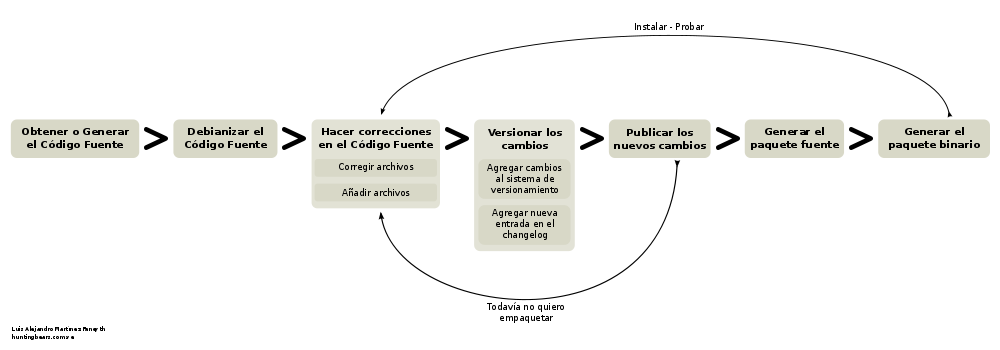
\includegraphics{diagrama2.png}


\subsection{Términos Fundamentales}

Para comenzar, primero debemos revisar algunos conceptos que nos ayudarán a desenvolvernos mejor en el ambiente de desarrollo que necesitaremos. Éstos términos serán descritos de forma que cualquiera lo pueda entender, puesto que es la introducción de éste post y a medida que vayas leyendo, el nivel de dificultad irá aumentando. Sin embargo, sólo se escribirá lo necesario para que empaquetes, es decir, nada faltará ni nada sobrará.


\bigskip\hrule{}\bigskip


Un \textbf{Paquete Fuente} (comúnmente de extensión .tar.gz) es un paquete comprimido que contiene los archivos fuente de un determinado software. Éstos pueden ser por sí mismos los archivos ejecutables (binarios, scripts, entre otros) o, pueden ser los archivos a través de los cuales se generan los ejecutables mediante de un proceso de compilación que depende directamente del lenguaje en que está escrito el software. Para que éstos archivos ejecutables (y demás archivos de contenido y configuración) sean reconocidos por el Sistema de Gestión de Paquetes de Debian, y gocen del beneficio que esto representa (tanto para el desarrollador como para el Sistema operativo), éstos deben ser agrupados y distribuidos a los usuarios en paquetes binarios (.deb).

Por otra parte, los paquetes fuente (adaptados a Debian GNU/Linux) contienen una carpeta llamada “debian” (nótese las minúsculas), en donde se encuentran diferentes archivos que contienen toda la información necesaria para generar el paquete binario a partir del código fuente. Comúnmente la generación de ésta carpeta (proceso al que se le llama “Debianización del Código Fuente”) es la parte más difícil del empaquetamiento, ya que se debe editar manualmente y para ello se debe conocer la estructura del Sistema Operativo (donde va cada tipo de cosa) y la estructura del programa que se desea empaquetar (para qué sirve cada cosa).

Los paquetes fuentes son distribuidos por el desarrollador de la aplicación y por el mantenedor del paquete en las diferentes distribuciones en las que esté disponible.


\bigskip\hrule{}\bigskip


Los \textbf{Paquetes Debian} (.deb), también llamados paquetes binarios, son paquetes que contienen software instalable en sistemas operativos Debian y derivados (Ubuntu, Canaima, etc...). Está compuesto por dos partes fundamentales: Archivos de Control y Archivos de Datos.

Los Archivos de Control están agrupados en una carpeta llamada “DEBIAN” (nótese las mayúsculas) y contienen la información necesaria para que el sistema de gestión de paquetes instale (control, md5sum) y configure el paquete (preinst, postinst, prerm, preinst); no debe ser confundido con la carpeta debian de los archivos fuente, la carpeta DEBIAN es generada a partir de la carpeta debian en el proceso de empaquetamiento.

Los Archivos de Datos son los archivos binarios, de texto, configuración y de contenido general propios de la aplicación, dispuestos en la estructura de archivos del sistema tal cual van a ser copiados.

Los paquetes binarios son distribuídos por el mantenedor (o empaquetador) de la aplicación en las diferentes distribuciones en las que esté disponible.


\bigskip\hrule{}\bigskip


Un \textbf{Makefile} es un archivo que forma parte de un paquete fuente y que contiene las instrucciones para probar, compilar, instalar, limpiar y desinstalar el software que se distribuye de forma “estática” (no recibe actualizaciones ni se verifican dependencias mediante el sistema de paquetes de Debian). Es generado por el desarrollador del software, quien conoce exactamente como realizar éstas operaciones.

En algunos casos más complejos, se hace necesario hacer un Makefile para distintos propósitos, por lo que se usa otro elemento que a partir de ciertos procedimientos, genera el Makefile automáticamente; éste elemento es el archivo configure. El archivo configure es producido por un set de herramientas desarrolladas por el proyecto GNU denominadas autotools (aunque también puede ser generado manualmente). Puedes encontrar mayor información de cómo generar el makefile para tus aplicaciones aquí, aquí, también aquí y probablemente aquí y aquí (también aquí, aquí, aquí y aquí).

El archivo rules de la carpeta debian es un archivo Makefile, que contiene las operaciones a realizar para generar la estructura de los Archivos de Datos de un paquete binario. Generalmente son operaciones comunes de movimiento de archivos, y creación de carpetas; sin embargo, pueden incluirse operaciones más complejas dependiendo de las necesidades del mantenedor del paquete. Recientemente, y gracias al conjunto de scripts debhelper, no es necesario realizar éstas operaciones “a mano” ya que existen “ayudantes” que detectan qué debe hacerse con cuales archivos a partir de la presencia de ciertas instrucciones en la carpeta debian durante el proceso de empaquetado. Puedes ampliar la información aquí.

Suficientes términos por ahora, manos a la obra!


\subsection{Empezando}

Para comenzar, necesitaremos varios insumos, uno de ellos es la descripción de nuestro entorno de trabajo. Estamos trabajando en el sistema operativo Canaima, sin embargo, ésta guía también es aplicable a sistemas operativos basados en Debian Lenny (con ligeras diferencias). Usaremos el paquete canaima-semilla para nuestro ejemplo.

Otra cosa que necesitaremos son herramientas de empaquetamiento. A continuación abran una terminal con permisos de Administrador y ejecuten el siguiente comando:

\begin{Verbatim}[commandchars=@\[\]]
aptitude install git-buildpackage build-essential dpkg-dev file libc6-dev patch perl autoconf automake dh-make debhelper devscripts devscripts-el fakeroot gnupg gpc xutils lintian cdbs pbuilder debian-policy developers-reference manpages-es manpages-es-extra debian-reference-es
\end{Verbatim}

Obteniendo el código fuente

Seguidamente obtengamos el código fuente de la aplicación a empaquetar, cosa que podemos hacer de dos formas:

1.- Clonando el repositorio git con el comando gpb-clone:

\begin{Verbatim}[commandchars=@\[\]]
gbp-clone git@PYGZat[]gitorious.org:canaima-gnu-linux/canaima-semilla.git
\end{Verbatim}

2.- O, generando un repositorio git local a partir de un paquete tar.gz:

\begin{Verbatim}[commandchars=@\[\]]
mkdir canaima-semilla
cd canaima-semilla
git init
git-import-orig canaima-semilla-1.5+3.orig.tar.gz
\end{Verbatim}

Luego de aplicado alguno de los métodos previos, tendremos una carpeta llamada “canaima-semilla”, conteniendo nuestro código fuente. Es una buena práctica renombar en ésta etapa la carpeta para que cumpla con el siguiente formato: \textless{}Paquete\textgreater{}-\textless{}Versión\textgreater{}+\textless{}Revisión\textgreater{}, para evitarnos problemas más adelante. En el caso de nuestro ejemplo quedaría: canaima-semilla-1.5+3.

Por supuesto, si se está empezando a escribir el programa desde cero, los métodos anteriores no son válidos, ya que ya tendríamos las fuentes en nuestro computador. En ese caso, simplemente posicionate en la carpeta raíz de tu proyecto y haz tu primera versión con git.


\subsection{Debianizando el código fuente}

Suponiendo que nuestro paquete no contiene la carpeta debian (generalmente se incluye) o que estamos haciendo un desarrollo nuevo (y no ha sido empaquetado antes), necesitaremos realizar éste trabajo por nosotros mismos mediante el comando dh\_make (debhelper). También, aunque ya tengamos la carpeta debian en nuestro código fuente, éste comando nos permite generar automáticamente una copia de las fuentes modificadas con el sufijo .orig, el cual es un elemento que será utilizado como insumo en un proceso posterior del empaquetado.

Como precaución, es recomendable declarar las siguientes variables de entorno antes de ejecutar el comando dh\_make, para asegurarnos de identificarnos bien:

\begin{Verbatim}[commandchars=@\[\]]
export DEBFULLNAME="@textless[]nombre completo del mantenedor@textgreater[]"
export DEBEMAIL="@textless[]correo del mantenedor@textgreater[]"
\end{Verbatim}

Estando dentro de la carpeta del paquete fuente, ejecutaremos el siguiente comando:

\begin{Verbatim}[commandchars=@\[\]]
dh@_make --createorig --cdbs --copyright @textless[]licencia@textgreater[] --email @textless[]correo@textgreater[]
\end{Verbatim}

En donde:
\begin{description}
\item[{\code{-{-}createorig}}] \leavevmode
Creará una copia de la carpeta donde se encuentra el código fuente, añadiendo el sufijo .orig. Ésto servirá para regenerar el paquete fuente en etapas posteriores del proceso.

\item[{\code{-{-}cdbs}}] \leavevmode
Le dirá al proceso que vamos a utilizar el Common Debian Build System, por lo que incluirá algunas plantillas útiles en la carpeta debian.

\item[{\code{-{-}copyright}}] \leavevmode
Especificará bajo cual licencia publicaremos nuestro software.

\item[{\code{-{-}email}}] \leavevmode
Identificará el código fuente con nuestro correo.

\end{description}

Para nuestro ejemplo haremos:

\begin{Verbatim}[commandchars=@\[\]]
dh@_make --createorig --cdbs --copyright gpl3 --email nombre@PYGZat[]correo.com
\end{Verbatim}

Una vez finalizado el proceso, tendremos unas fuentes debianizadas. Sin embargo, ahora hay que adaptarlas a las necesidades del paquete binario que queremos construir. Examinemos lo que ha puesto dh\_make en la carpeta debian por nosotros:
\begin{itemize}
\item {} 
changelog

\item {} 
compat

\item {} 
control

\item {} 
copyright

\item {} 
cron.d.ex

\item {} 
docs

\item {} 
emacsen-install.ex

\item {} 
emacsen-remove.ex

\item {} 
emacsen-startup.ex

\item {} 
init.d.ex

\item {} 
manpage.1.ex

\item {} 
manpage.sgml.ex

\item {} 
manpage.xml.ex

\item {} 
menu.ex

\item {} 
postinst.ex

\item {} 
postrm.ex

\item {} 
preinst.ex

\item {} 
prerm.ex

\item {} 
prueba.cron.d.ex

\item {} 
prueba.default.ex

\item {} 
prueba.doc-base.EX

\item {} 
README.source

\item {} 
README.Debian

\item {} 
rules

\item {} 
source

\item {} 
watch.ex

\end{itemize}

Cada uno de éstos archivos son utilizados por algún ayudante de debhelper para construir el paquete. Su configuración es bastante intuitiva, sin embargo proporcionamos algunos ejemplos:
\begin{quote}\begin{description}
\item[{debian/control}] \leavevmode
Este archivo controla el nombre del paquete fuente, el nombre del paquete binario, en qué sección va el paquete, quién es el responsable (aquí podemos definir también co-responsables), si el paquete reemplaza a otro, sugerir y/o recomendar otras cosas y definir dependencias (tanto en fuentes como en binarios). Más información…

\item[{debian/changelog}] \leavevmode
En este archivo verás el paquete, la versión+revisión Debian, repositorio y la urgencia, algo como canaima-semilla (1.5+3) desarrollo; urgency=low. Donde 1.5 es la versión del programa, +3 es la revisión de Debian, desarrollo es el repositorio al que deberías subirlo y urgency=low establece cuánto tiempo pasará en paquete en «desarrollo» antes de que se intente migrar a «pruebas» («low» significa 10 días), normalmente usarás el valor «low», aunque «medium» y «high» también están disponibles.

\item[{debian/copyright}] \leavevmode
En este archivo debes especificar el autor original, el lugar desde el que descargaste el software, y la licencia del programa. Más información…

\item[{debian/docs}] \leavevmode
Este archivo incluye los documentos que se copiarán a /usr/share/doc/paquete cuando se instale. Deben incluirse uno por línea.

\item[{debian/compat}] \leavevmode
Este archivo determina el nivel de compatibilidad con debhelper. Actualmente el nivel recomendado es 7.

\end{description}\end{quote}


\subsection{Realizar cambios al código fuente}

Ésta etapa es bastante flexible y depende en su totalidad de la persona que lo haga. Aquí se harán los cambios que el desarrollador considere de acuerdo con sus objetivos (corregir errores, agregar funcionalidades, entre otros). Usará las herramientas que considere necesarias e incorporará y modificará los archivos que desee sin ningún tipo de restricción, siempre y cuando lo haga dentro de la carpeta de trabajo e incorpore las nuevas reglas (si las hubiera) en los archivos de construcción e instalación del paquete (Makefile, debian/rules, etc..).


\subsection{Versionar los cambios}

Una vez realizados los cambios, y se considere que son suficientes como para que constituyan una nueva versión de nuestro paquete, es tiempo de versionar el nuevo estado de tu proyecto. Para ello utilizaremos el flujo de trabajo natural de git, que describimos en un post anterior, para luego plasmar los cambios en el archivo debian/changelog mediante el comando git-dch. Éste comando se encargará de recopilar todos los commits nuevos que se han hecho desde la última versión y usará todos sus mensajes para llenar el archivo debian/changelog con una nueva entrada.

Como precaución, es recomendable declarar las siguientes variables de entorno antes de ejecutar el comando git-dch, para asegurarnos de identificarnos bien:

\begin{Verbatim}[commandchars=@\[\]]
export DEBFULLNAME="@textless[]nombre completo del mantenedor@textgreater[]"
export DEBEMAIL="@textless[]correo del mantenedor@textgreater[]"
\end{Verbatim}

Ejecutamos en el directorio base, el siguiente comando:

\begin{Verbatim}[commandchars=\\\{\}]
\PYG{n}{git}\PYG{o}{-}\PYG{n}{dch} \PYG{o}{-}\PYG{o}{-}\PYG{n}{release} \PYG{o}{-}\PYG{o}{-}\PYG{n}{auto} \PYG{o}{-}\PYG{o}{-}\PYG{n+nb}{id}\PYG{o}{-}\PYG{n}{length}\PYG{o}{=}\PYG{l+m+mi}{7} \PYG{o}{-}\PYG{o}{-}\PYG{n}{full}
\end{Verbatim}

En donde:
\begin{description}
\item[{\code{-{-}release}}] \leavevmode
Indica que es una nueva versión y que es definitiva (si en cambio usamos –snapshot, se considerará como una versión temporal)

\item[{\code{-{-}auto}}] \leavevmode
Indica que se adivinará el número de la versión a partir de la entrada anterior.

\item[{\code{-{-}id-length="N"}}] \leavevmode
Es el número de caracteres del código del commit que se incluirán.

\item[{\code{-{-}full}}] \leavevmode
Le indicará que debe incluir todo el mensaje del commit y no un extracto del mismo.

\end{description}

Si por casualidad hemos ejecutado éste comando sin tener commits nuevos, la nueva entrada del debian/changelog será rellenada con la palabra “UNRELEASED”, la cual desaparecerá en el próximo ciclo de versionamiento.


\subsection{Generar el paquete fuente}

Para generar el paquete fuente, necesitamos añadir los cambios a la rama upstream, la cual es usada como rama “fuente”. Si no está disponible debemos crearla con el comando \textbf{git branch upstream}. Para añadir los cambios debemos fusionar la rama master con la upstream de la siguiente forma:

\begin{Verbatim}[commandchars=@\[\]]
git checkout upstream
git merge master
git checkout master
\end{Verbatim}

El siguiente paso es generar la carpeta .orig.tar.gz que va a ser utilizada para generar el paquete fuente, a través de dh-make:

\begin{Verbatim}[commandchars=@\[\]]
dh@_make --createorig --cdbs --copyright @textless[]licencia@textgreater[] --email @textless[]correo@textgreater[]
\end{Verbatim}

Seguidamente, creamos el paquete fuente en cuestión, excluyendo el directorio git:

\begin{Verbatim}[commandchars=@\[\]]
cd ..
dpkg-source --format="1.0" -i.git/ -I.git -b canaima-semilla-1.5+3
\end{Verbatim}


\subsection{Publicar los cambios}

En ésta etapa, es hora de hacer saber a los demás que existe una nueva versión del código fuente, y la mejor forma de hacerlo es a través de un repositorio público como github o gitorious.
\begin{quote}

git push origin master upstream
\end{quote}


\subsection{Generar el paquete binario}

Finalmente podemos generar nuestro paquete binario. Para ello ejecutamos el siguiente comando:

\begin{Verbatim}[commandchars=\\\{\}]
\PYG{n}{git}\PYG{o}{-}\PYG{n}{buildpackage} \PYG{o}{-}\PYG{n}{k}\PYG{o}{\textless{}}\PYG{n}{llave}\PYG{o}{\textgreater{}} \PYG{o}{-}\PYG{n}{tc} \PYG{o}{-}\PYG{o}{-}\PYG{n}{git}\PYG{o}{-}\PYG{n}{tag} \PYG{o}{-}\PYG{n}{jN}
\end{Verbatim}

En donde:
\begin{description}
\item[{\code{-k\textless{}llave\textgreater{}}}] \leavevmode
Especifica la llave pública GPG con que se firmará el paquete.

\item[{\code{-tc}}] \leavevmode
Limpia el directorio base de los residuos de la construcción del paquete.

\item[{\code{-{-}git-tag}}] \leavevmode
Crea una etiqueta que agrupa todos los commits de una determinada versión.

\item[{\code{-jN}}] \leavevmode
Permite utilizar un número N de hilos para ejecutar el proceso. Se recomienda que N sea el número de procesadores más uno.

\end{description}

Si el proceso culmina satisfactoriamente, correrá lintian para indicarnos si hay alguna discrepancia con las normas de empaquetamiento de debian.

Si el proceso se interrumpe, es una buena práctica crear el tag para evitar errores al correr git-dch en el próximo ciclo. Ejecuta \code{gitbuildpackage -{-}git-tag-only} para asignar el tag sin volver a intentar construir el paquete.


\subsection{Hoja Resumen (cheat sheet) del flujo de trabajo}

\begin{Verbatim}[commandchars=@\[\]]
git add .
git commit --all
git-dch --release --auto --id-length=7 --full
(directorio renombrado)
cd ../nuevo-directorio/
git commit --all
git checkout upstream
git merge master
git checkout master
git push origin master upstream
dh@_make --createorig --cdbs --copyright @textless[]licencia@textgreater[] --email @textless[]correo@textgreater[]
cd ..
(para crear las fuentes formato 1.0)
dpkg-source --format="1.0" -i.git/ -I.git -b nuevo-directorio
cd nuevo-directorio
git push gitorious master upstream
git-buildpackage -k@textless[]llave@textgreater[] -tc --git-tag -jN
\end{Verbatim}

¡Feliz Empaquetado!

\resetcurrentobjects
\hypertarget{--doc-guia-referencia}{}

\chapter{\textbf{Guía de Referencia para el Desarrollador}}

Este documento tratará de describir cómo se construye un paquete Canaima GNU/Linux para el usuario común de Canaima y para futuros desarrolladores en un lenguaje informal, y con multitud de ejemplos. Hay un antiguo dicho romano que dice, Longum iter est per preaecepta, breve et efficax per exempla! (¡Es un largo camino con las reglas, pero corto y eficiente con ejemplos!)

Canaima esta basado en Debian, y una de las cosas que hace a Debian una de las distribuciones más importantes del mercado es su sistema de paquetes. Aunque hay una gran cantidad de programas disponibles en forma de paquetes de Debian, algunas veces necesitarás instalar programas que no están disponible en este formato.

Este documento explicará cada pequeño paso (al principio quizás irrelevantes), le ayudará a crear tu primer paquete, ganar alguna experiencia en construir próximas versiones de él, y quizás otros paquetes después.

Este documento se basa en la ``Guía del nuevo desarrollador de Debian''. se pueden obtener versiones nuevas de este documento en línea en \href{http://www.debian.org/doc/maint-guide/}{http://www.debian.org/doc/maint-guide/} y en el paquete «maint-guide-es».


\section{\textbf{Programas que necesitas para el desarrollo}}

Antes de empezar nada, deberías asegurarte de que tienes instalados algunos paquetes adicionales necesarios para el desarrollo. Observa que en la lista no están incluidos paquetes cuyas prioridades son «esencial» o «requerido», que se suponen ya instalados.

Los siguientes paquetes vienen en una instalación estándar de Canaima, así que probablemente ya los tengas (junto con los paquetes de los que dependen). Aún así, deberías comprobarlo con:

\begin{Verbatim}[commandchars=@\[\]]
dpkg -s @textless[]paquete@textgreater[]
\end{Verbatim}
\begin{quote}\begin{description}
\item[{dpkg-dev}] \leavevmode
este paquete contiene las herramientas necesarias para desempaquetar, construir y enviar paquetes fuente de Canaima.

\item[{file}] \leavevmode
este útil programa puede determinar de qué tipo es un fichero

\item[{gcc}] \leavevmode
el compilador de C de GNU, necesario si el programa, como la gran mayoría, está escrito en el lenguaje de programación C. Este paquete también vendrá con otros paquetes como \textbf{binutils} que incluye programas para ensamblar y enlazar ficheros objeto y el preprocesador de C en el paquete cpp.

\item[{libc6-dev}] \leavevmode
las bibliotecas y archivos de cabecera de C que gcc necesita para enlazar y crear ficheros objeto.

\item[{make}] \leavevmode
habitualmente la creación de un programa consta de varios pasos. En lugar de ejecutar las mismas órdenes una y otra vez, puedes utilizar este programa para automatizar el proceso, creando ficheros \textbf{«Makefile»}

\item[{patch}] \leavevmode
esta utilidad es muy práctica, ya que permite tomar un fichero que contiene un listado de diferencias (producido por el programa diff) y aplicárselas al fichero original, produciendo una versión ``parcheada''.

\item[{perl}] \leavevmode
Perl es uno de los lenguajes interpretados para hacer guiones (o \emph{«scripts»}) más usados en los sistemas Un*x de hoy en día, comúnmente se refiere a él como la \textbf{«navaja suiza de Unix»}.

\end{description}\end{quote}

\emph{Probablemente, necesitarás instalar además los siguientes paquetes:}

\emph{autoconf} y \emph{automake}: muchos programas nuevos usan ficheros de configuración y ficheros «Makefile» que se procesan con la ayuda de programas como éstos.

\emph{dh-make} y \emph{debhelper}: \emph{dh-make} es necesario para crear el esqueleto de nuestro paquete ejemplo, y se usarán algunas de las herramientas de debhelper para crear los paquetes. Aunque no son imprescindibles para la creación de paquetes se recomiendan encarecidamente para nuevos desarrolladores. Hacen el proceso mucho más fácil al principio, y más fácil de controlar también más adelante, mas información en el directorio \emph{/doc/debhelper/README}.

\emph{devscripts}: este paquete contiene algunos guiones útiles para los desarrolladores, pero no son necesarios para crear paquetes, mas información en el directorio \emph{/usr/share/doc/devscripts/README.gz}.

\emph{fakeroot}: esta utilidad te permite emular al usuario administrador (o \emph{root}), lo cual es necesario para ciertas partes del proceso de construcción.

\emph{gnupg}: herramienta que te permite firmar digitalmente los paquetes. Esto es especialmente importante si quieres distribuir tu paquete a otras personas, y ciertamente, tendrás que hacerlo cuando tu trabajo vaya a incluirse en la distribución de Debian.

\emph{g77}: el compilador GNU de Fortran 77, necesario si el programa está escrito en Fortran.

\emph{gpc}: el compilador GNU de Pascal, necesario si el programa está escrito en Pascal. Merece la pena mencionar aquí fp-compiler, un compilador libre de Pascal, que también es bueno en esta tarea.

\emph{xutils}: algunos programas, normalmente aquellos hechos para X11, también usan programas para generar Makefiles de un conjunto de funciones de macro.

\emph{lintian}: este es el comprobador de paquetes de Debian, que te indica muchos de los errores comunes después de construir un paquete, y explica los errores encontrados, mas información en \emph{/usr/share/doc/lintian/lintian.html/index.html}.

\emph{pbuilder}: este paquete contiene programas para crear y mantener entornos chroot. Al construir paquetes Debian en estos entornos chroot se verifica que las dependencias son las adecuadas y se evitan fallos al construir desde el código fuente.

Las breves descripciones dadas anteriormente sólo sirven para introducirte a lo que hace cada paquete. Antes de continuar, por favor, lee la documentación de cada programa, al menos para su uso normal. Puede parecerte algo duro ahora, pero más adelante estarás muy contento de haberla leído.
Nota: debmake es un paquete que incluye otros programas con funciones similares a dh-make, pero su uso específico no está cubierto en este documento porque se trata de una herramienta obsoleta.


\section{\textbf{Desarrollador oficial de Canaima}}

Puede que te quieras convertir en un desarrollador oficial de Canaima una vez hayas construido tu paquete (o incluso mientras lo estás haciendo) para que el paquete se introduzca en la nueva distribución (si el programa es útil, ¿por qué no?).

No puedes convertirte en desarrollador oficial de Canaima de la noche a la mañana porque hace falta más que sólo habilidades técnicas. No te sientas desilusionado por esto. Aún puedes subir tu paquete, si es útil a otras personas, como su mantenedor a través de un patrocinador mientras tu entras en el proceso de nuevos desarrolladores de Debian. En este caso el patrocinador es un desarrollador oficial de Debian que ayuda a la persona que mantiene el paquete a subirlo al archivo de Debian.

Ten en cuenta que no tienes que crear un paquete nuevo para poder convertirte en desarrollador oficial. Un camino posible para ser desarrollador oficial es contribuir al mantenimiento de los paquetes ya existentes en la distribución.


\subsection{Más información}

Puedes construir dos tipos de paquetes: fuentes y binarios. Un paquete fuente contiene el código que puedes compilar en un programa. Un paquete binario contiene sólo el programa terminado. ¡No mezcles los términos como «fuentes de un programa» y el «paquete fuente de un programa»! Por favor, lee los otros manuales si necesitas más detalles sobre terminología.

Canaima usa el término \emph{desarrollador} se utiliza para referirse a la persona que hace paquetes, y el termino \emph{autor original} para la persona que hizo el programa, y \emph{desarrollador original} para la persona que actualmente mantiene el programa fuera de Debian. Generalmente el autor y el desarrollador fuente son la misma persona - y algunas veces incluso el desarrollador es el mismo. Si haces un programa, y quieres incluirlo en Debian, tienes total libertad para solicitar convertirte en desarrollador.


\section{\textbf{Primeros Pasos}}


\subsection{Elige el programa}

Probablemente hayas escogido ya el paquete que deseas construir. Lo primero que debes hacer es comprobar si el paquete está ya en el archivo de la distribución utilizando synaptic.

Si el paquete es nuevo y decides que te gustaría verlo en Canaima GNU/Linux debes seguir los pasos indicados a continuación:
\begin{itemize}
\item {} 
Comprueba que no hay nadie más trabajando ya en el paquete consultando la lista de paquetes en los que se está trabajando. Si ya hay alguien trabajando en él, contacta con esa persona. Si no, intenta encontrar otro programa interesante que nadie mantenga.

\item {} 
El programa debe tener una licencia. Preferiblemente la licencia deberá ser libre en el sentido marcado por las Directrices de Debian para el software libre y no puede depender de un paquete que no esté dentro de «main» para compilarse o para poder utilizarse. Si la licencia no sigue alguna de estas reglas aún puede incluirse en las secciones «contrib» o «non-free» de Debian dependiendo de su situación. Si no estás seguro sobre en qué lugar debería ir, envía el texto de la licencia y pide consejo con un correo (en inglés) dirigido a \href{mailto:debian-legal@lists.debian.org}{debian-legal@lists.debian.org}.

\item {} 
El programa no debería ejecutarse con «setuid root», o aún mejor: no debería ser «setuid» ni «setgid».

\item {} 
El programa no debería ser un demonio, o algo que vaya en los directorios \emph{/sbin}, o abrir un puerto como usuario administrador.

\item {} 
El programa debería estar compuesto por binarios ejecutables, no intentes empaquetar aún con bibliotecas.

\item {} 
El programa debería tener una buena documentación, o al menos un código fuente legible y no ofuscado.

\item {} 
Deberías contactar con el autor o autores del programa para comprobar si está/n de acuerdo con que se empaquete. Es importante que el autor o autores sigan manteniendo el programa para que puedas en el futuro consultarle/s en caso de que haya problemas específicos. No deberías intentar empaquetar programas que no estén mantenidos.

\item {} 
Y por último, pero no menos importante, deberías saber cómo funciona, y haberlo utilizado durante algún tiempo.

\end{itemize}

Por supuesto, esta lista es para tomar medidas de seguridad, y con la intención de salvarte de usuarios enfurecidos si haces algo mal con algún demonio «setuid»... Cuando tengas más experiencia en empaquetar, podrás hacer este tipo de paquetes, incluso los desarrolladores más experimentados preguntan en la lista de correo de \emph{desarrolladores} cuando tienen dudas. La gente allí te ayudará gustosamente.


\subsection{Obtén el programa y pruébalo}

Lo primero que debes hacer es encontrar y descargar el paquete original. A partir de este punto se da por supuesto que ya tienes el código fuente que obtuviste de la página del autor. Las fuentes de los programas libres de GNU/Linux generalmente vienen en formato \emph{tar/gzip}, con extensión \emph{.tar.gz}, y generalmente contienen un subdirectorio llamado \emph{«programa-versión»} con todas las fuentes en él. Si tu programa viene en otro tipo de archivo (por ejemplo, el fichero termina en ``.Z'' o ``.zip''), descomprímelo con las herramientas adecuadas, o pregunta en la lista de correo \emph{desarrolladores} si tienes dudas de cómo se puede desempaquetar correctamente (pista: prueba \emph{«file archivo.extensión»}).

Como ejemplo, usaré el programa conocido como «gentoo», un gestor de ficheros de X11 en GTK+. Observa que el programa ya ha sido empaquetado previamente pero ha cambiado sustancialmente de versión desde que este texto se escribió.

Crea un subdirectorio bajo tu directorio personal llamado «debian» o «deb» o lo que creas apropiado (por ejemplo \textasciitilde{}/gentoo/ estaría bien en este caso). Mueve a él el archivo que has descargado, y descomprímelo de la siguiente forma: «tar xzf gentoo-0.9.12.tar.gz». Asegúrate de que no hay errores, incluso errores «irrelevantes», porque es muy probable que haya problemas al desempaquetarlo en sistemas de otras personas, cuyas herramientas de desempaquetado puede que no ignoren estas anomalías.

Ahora tienes otro subdirectorio, llamado «gentoo-0.9.12». Muévete a ese directorio y lee en profundidad la documentación que encuentres. Generalmente se encuentra en ficheros que se llaman \emph{README}, \emph{INSTALL}, *.lsm o *.html. Allí encontrarás instrucciones de cómo compilar e instalar el programa (muy probablemente asumirán que lo quieres instalar en el directorio /usr/local/bin, no harás esto, pero eso lo veremos más adelante en Instalación en un subdirectorio, Sección 3.1).

El proceso varía de un programa a otro, pero gran parte de los programas modernos vienen con un guión \emph{«configure»} que configura las fuentes para tu sistema y se asegura de que el sistema está en condiciones de compilarlo. Después de configurarlo (con \emph{«./configure»}), los programas generalmente se compilan con \emph{«make»}. Algunos de ellos soportan \emph{«make check»} para ejecutarse incluyendo comprobaciones automáticas. Generalmente se instalarán en sus directorios de destino ejecutando \emph{«make install»}.

Ahora intenta compilar, y ejecutar el programa, para asegurarte de que funciona bien y de que no rompe nada mientras está instalándose o ejecutándose.

También, generalmente, puedes ejecutar \emph{«make clean»} (o mejor \emph{«make distclean»}) para limpiar el directorio donde se genera el programa. A veces hay incluso un \emph{«make uninstall»} que se puede utilizar para borrar todos los archivos instalados.


\subsection{Nombre del paquete y versión}

Deberías empezar a construir tu paquete en un directorio de fuentes completamente limpio, o simplemente con las fuentes recién desempaquetadas.

Para construir correctamente el paquete, debes cambiar el nombre original del programa a letras minúsculas (si no lo está ya), y deberías renombrar el directorio de fuentes a \emph{\textless{}nombre\_de\_paquete\textgreater{}-\textless{}versión\textgreater{}}.

Si el nombre del programa está formado por varias palabras, contráelas a una palabra o haz una abreviatura. Por ejemplo, el paquete del programa «el editor para X de Javi» se podría llamar javiedx o jle4x, o lo que decidas, siempre y cuando no se exceda de unos límites razonables, como 20 caracteres.

Comprueba también la versión exacta del programa (la que se incluye en la versión del paquete). Si el programa no está numerado con versiones del estilo de X.Y.Z, pero sí con fecha de publicación, eres libre de utilizar la fecha como número de versión, precedida por «0.0» (sólo por si los desarrolladores originales deciden sacar una versión nueva como 1.0). Así, si la fecha de las fuentes es el 19 de diciembre de 1998, puedes utilizar la cadena 0 0.0.19981219 (que utiliza el formato de fecha ISO 8601, N. del T.) como número de versión.

Aún así habrá algunos programas que ni siquiera estén numerados, en cuyo caso deberás contactar con el desarrollador original para ver si tienen algún otro sistema de seguimiento de revisiones.


\subsection{«Debianización» inicial}

Asegúrate que te encuentras en el directorio donde están las fuentes del programa y ejecuta lo siguiente:

\begin{Verbatim}[commandchars=@\[\]]
dh@_make -e tu.dirección@PYGZat[]de.desarrollador -f ../gentoo-0.9.12.tar.gz
\end{Verbatim}

Por supuesto, cambia la cadena «tu.dirección@de.desarrollador» por tu dirección de correo electrónico para que se incluya en la entrada del fichero de cambios así como en otros ficheros, y el nombre de fichero de tu archivo fuente original.

Saldrá alguna información. Te preguntará qué tipo de paquete deseas crear. Gentoo es un sólo paquete de binarios - crea sólo un binario, y, por tanto, sólo un fichero .deb - así que seleccionaremos la primera opción, con la tecla «s». Comprueba la información que aparece en la pantalla y confirma pulsando la tecla \textless{}intro\textgreater{}.

Tras ejecutar dh\_make, se crea una copia del código original con el nombre gentoo\_0.9.12.orig.tar.gz en el directorio raíz para facilitar la creación del paquete de fuentes no nativo de Debian con el diff.gz. Observa que hay dos cambios clave en este nombre de fichero:
\begin{itemize}
\item {} 
El nombre del paquete y la versión están separados por «\_».

\item {} 
Hay un «orig.» antes de «tar.gz».

\end{itemize}

Como nuevo desarrollador, se desaconseja crear paquetes complicados, por ejemplo:
\begin{itemize}
\item {} 
múltiples paquetes binarios

\item {} 
paquetes de bibliotecas

\item {} 
paquetes en los que el formato del archivo fuente no es en tar.gz. ni en tar.bz2, o

\item {} 
paquetes cuyas fuentes contienen partes que no se pueden distribuir.

\end{itemize}

Estos casos no son extremadamente difíciles, pero sí necesita algunos conocimientos más, así que aquí no se describirá el proceso de empaquetado para este tipo de paquetes.

Ten en cuenta que deberías ejecutar dh\_make sólo una vez, y que no se comportará correctamente si lo haces otra vez en el mismo directorio ya «debianizado». Esto también significa que usarás un método distinto para crear una nueva revisión o una nueva versión de tu paquete en el futuro.


\subsection{Modificar las fuentes}

Por lo general, los programas se instalan a sí mismos en el subdirectorio /usr/local. Pero los paquetes Debian no pueden utilizar este directorio ya que está reservado para el uso privado del administrador (o de los usuarios). Esto significa que tienes que mirar el sistema de construcción de tu programa, generalmente empezando por el fichero \emph{«Makefile»}. Éste es el guión \emph{make} que se usará para automatizar la creación de este programa.

Observa que si tu programa usa GNU automake y/o autoconf, lo que quiere decir que las fuentes incluyen ficheros Makefile.am y Makefile.in, respectivamente, ya que necesitarás modificar esos ficheros, porque cada invocación de \emph{automake} reescribirá los ficheros \emph{«Makefile.in»} con información generada a partir de los ficheros \emph{«Makefile.am»}, y cada llamada a \emph{./configure} hará lo mismo con los ficheros \emph{«Makefile»}, con información de los ficheros \emph{«Makefile.in»}. Editar los ficheros \emph{«Makefile.am»} requiere algunos conocimientos de \emph{automake}, que puedes obtener leyendo la entrada de \emph{info} para \emph{automake}, mientras que editar los ficheros \emph{«Makefile.in»} es casi lo mismo que editar ficheros \emph{«Makefile»}, simplemente basta con poner atención en las variables, es decir, cualquier cadena que empiece y acabe con el caracter «@», como por ejemplo @CFLAGS@ o @LN\_S@, que se sustituyen por otros valores cada vez que se ejecute \emph{./configure}. Por favor, lee \emph{/usr/share/doc/autotools-dev/README.Debian.gz} antes de empezar.

Ten en cuenta que no hay espacio aquí para entrar en todos los detalles respecto a los arreglos que deben hacerse en las fuentes originales. Sin embargo, a continuación se detallan algunos de los problemas más frecuentes.


\subsection{Instalación en un subdirectorio}

La mayor parte de los programas tienen alguna manera de instalarse en la estructura de directorios existente en tu sistema, para que los binarios sean incluidos en tu \emph{\$PATH}, y para que encuentre la documentación y páginas de manual en los lugares habituales. Sin embargo, si lo instalas de esta forma, el programa se instalará con los demás binarios que ya están en tu sistema. Esto dificultará a las herramientas de paquetes averiguar qué archivos pertenecen a tu paquete y cuales no.

Por lo tanto, necesitas hacer algo más: instalar el programa en un subdirectorio temporal desde el cual las herramientas de desarrollo construirán el paquete \emph{.deb} que se pueda instalar. Todo lo que se incluye en este directorio será instalado en el sistema del usuario cuando instale su paquete, la única diferencia es que \emph{dpkg} instalará los ficheros en el directorio raíz.

Este directorio temporal se creará bajo el directorio \emph{debian/} que está dentro del árbol del código descomprimido, generalmente con el nombre \emph{debian/nombre\_de\_paquete.}

Ten en cuenta que, aunque necesitas que el programa se instale en \emph{debian/nombre\_de\_paquete}, también necesitas que se comporte correctamente cuando se instale en el directorio raíz, es decir, cuando se instale desde el paquete \emph{.deb}. Así que no deberías permitir que al construirse lo haga con cadenas como \emph{/home/canaima/deb/gentoo-0.9.12/usr/share/gentoo} dentro de los archivos del paquete a distribuir.

Esto será sencillo con los de programas que utilicen la herramienta GNU \emph{autoconf}. La mayoría de estos programas tienen ficheros \emph{«Makefile»} por omisión que permiten configurar la instalación en un subdirectorio cualquiera, aunque recordando que, por ejemplo, \emph{/usr} es el prefijo normal. Cuando detecte que tu programa usa \emph{autoconf}, \emph{dh\_make} fijará las opciones necesarias para hacer esto automáticamente, así que puedes dejar de leer esta sección. Pero con otros programas puede ser necesario que examines y edites los ficheros \emph{«Makefile»}.

Esta es la parte importante del \emph{Makefile} de gentoo:

\begin{Verbatim}[commandchars=@\[\]]
@# ¿Dónde poner el binario cuando se ejecute «make install»?
BIN     = /usr/local/bin

@# ¿Dónde poner los iconos cuando se ejecute «make install»?
ICONS   = /usr/local/share/gentoo/
\end{Verbatim}

Vemos que los ficheros están configurados para instalarse bajo /usr/local. Cambia estas rutas a:

\begin{Verbatim}[commandchars=@\[\]]
@# ¿Dónde poner el binario cuando se ejecute «make install»?
BIN     = @$(DESTDIR)/usr/bin

@# ¿Dónde poner los iconos cuando se ejecute «make install»?
ICONS   = @$(DESTDIR)/usr/share/gentoo
\end{Verbatim}

Pero: ¿por qué en este directorio y no en otro? Porque los paquetes de Debian nunca se instalan bajo \emph{/usr/local}, este árbol de directorio, está reservado para el uso del administrador del sistema. Así que estos ficheros deben instalarse en \emph{/usr}.

La localización correcta de los binarios, iconos, documentación, etc, está especificada en el \emph{«Estándar de la jerarquía del sistema de ficheros»} (véase \emph{/usr/share/doc/debian-policy/fhs}). Te recomiendo que leas las secciones que podrían aplicar a tu paquete.

Así pues, deberíamos instalar el binario en \emph{/usr/bin} en lugar de \emph{/usr/local/bin} y la página de manual en \emph{/usr/share/man/man1} en lugar de \emph{/usr/local/man/man1}. No hemos mencionado ninguna página de manual en el \emph{Makefile} de gentoo, pero en Debian se requiere que cada programa debe tener una, así que haremos una más tarde y la instalaremos en /usr/share/man/man1.

Algunos programas no usan variables en el \emph{makefile} para definir rutas como éstas. Esto significa que tendrás que editar algunos de los ficheros de código C para arreglarlos y que usen las rutas correctas. Pero, ¿dónde buscar?, y exactamente, ¿el qué? Puedes probar a encontrarlos usando:

\begin{Verbatim}[commandchars=@\[\]]
grep -nr -e 'usr/local/lib' --include='*.@PYGZlb[]c@textbar[]h@PYGZrb[]' .
\end{Verbatim}

(En cada subdirectorio que contenga ficheros .c y .h, grep nos indicará el nombre del fichero y la línea cuando encuentre una ocurrencia.

Ahora edita esos ficheros y cambia en esas líneas \emph{usr/local/lib} con \emph{usr/share} y ya está. Sólo tienes que reemplazar \emph{usr/local/lib} por tu localización, pero debes ser muy cuidadoso para no modificar el resto del código, especialmente si no sabes mucho sobre cómo programar en C.

Después de esto deberías encontrar el objetivo \emph{«install»} (busca una línea que comience por \emph{«install:»}) y renombra todas las referencias a directorios distintos de los definidos al comienzo del \emph{Makefile}. Anteriormente el objetivo \emph{«install»} decía:

\begin{Verbatim}[commandchars=@\[\]]
install:        gentoo
                install ./gentoo @$(BIN)
                install icons @$(ICONS)
                install gentoorc-example @$(HOME)/.gentoorc
\end{Verbatim}

Después del cambio dice:

\begin{Verbatim}[commandchars=@\[\]]
install:        gentoo-target
                install -d @$(BIN) @$(ICONS) @$(DESTDIR)/etc
                install ./gentoo @$(BIN)
                install -m644 icons/* @$(ICONS)
                install -m644 gentoorc-example @$(DESTDIR)/etc/gentoorc
\end{Verbatim}

Seguramente has notado que ahora hay una orden \emph{install -d} antes de las demás órdenes de la regla. El \emph{makefile} original no lo tenía porque normalmente \emph{/usr/local/bin} y otros directorios ya existen en el sistema donde se ejecuta \emph{«make install»}. Sin embargo, dado que lo instalaremos en un directorio vacío (o incluso inexistente), tendremos que crear cada uno de estos directorios.

También podemos añadir otras cosas al final de la regla, como la instalación de documentación adicional que los desarrolladores originales a veces omiten:

\begin{Verbatim}[commandchars=@\[\]]
install -d @$(DESTDIR)/usr/share/doc/gentoo/html
cp -a docs/* @$(DESTDIR)/usr/share/doc/gentoo/html
\end{Verbatim}

Un lector atento se dará cuenta de que he cambiado \emph{«gentoo»} a \emph{«gentoo-target»} en la línea \emph{«install:»}. A eso se le llama arreglar un fallo en el programa.

Siempre que hagas cambios que no estén específicamente relacionados con el paquete Debian, asegúrate de que los envías al desarrollador original para que éste los pueda incluir en la próxima revisión del programa y así le puedan ser útiles a alguien más. Además, recuerda hacer que tus cambios no sean específicos para Debian o Linux (¡ni siquiera para Unix!) antes de enviarlos, hazlo portable. Esto hará que tus arreglos sean más fáciles de aplicar.

Ten en cuenta que no tienes que enviar ninguno de los ficheros debian/* al desarrollador original.


\subsection{Bibliotecas diferentes}

Hay otro problema común: las bibliotecas son generalmente diferentes de plataforma a plataforma. Por ejemplo, un \emph{Makefile} puede contener una referencia a una biblioteca que no exista en Debian o ni siquiera en Linux. En este caso, se necesita cambiarla a una biblioteca que sí exista en Debian y sirva para el mismo propósito.

Así, si hay una línea en el \emph{Makefile} (o Makefile.in) de tu programa que dice algo como lo siguiente (y tu programa no compila):

\begin{Verbatim}[commandchars=@\[\]]
LIBS = -lcurses -lcosas -lmáscosas
\end{Verbatim}

Entonces cámbiala a lo siguiente, y funcionará casi con seguridad:

\begin{Verbatim}[commandchars=@\[\]]
LIBS = -lncurses -lcosas -lmáscosas
\end{Verbatim}

(El autor se ha dado cuenta de que éste no es el mejor ejemplo ya que ahora el paquete libncurses incluye un enlace simbólico a libcurses.so, pero no puedo pensar uno mejor. Cualquier sugerencia sería muy bien recibida :-)


\section{\textbf{Las cosas necesarias bajo debian}}

Ahora hay un nuevo subdirectorio bajo el directorio principal del programa (\emph{«gentoo-0.9.12»}), que se llama \emph{«debian»}. Hay algunos ficheros en este directorio que debemos editar para adaptar el comportamiento del paquete. La parte más importante es modificar los ficheros \emph{«control»}, \emph{«rules»}, \emph{«changelog»}, y \emph{«copyright»} que son necesarios en todos los paquetes.


\subsection{El fichero «control»}

Este fichero contiene varios valores que \emph{dpkg}, \emph{dselect} y otras herramientas de gestión de paquetes usarán para gestionar el paquete.

Aquí está el fichero de control que dh\_make crea para nosotros:

\begin{Verbatim}[commandchars=@\[\]]
1  Source: gentoo
2  Section: unknown
3  Priority: optional
4  Maintainer: Josip Rodin @textless[]joy-mg@PYGZat[]debian.org@textgreater[]
5  Build-Depends: debhelper (@textgreater[]@textgreater[] 3.0.0)
6  Standards-Version: 3.6.2
7
8  Package: gentoo
9  Architecture: any
10 Depends: @${shlibs:Depends}
11 Description: @textless[]insertar hasta 60 caracteres de descripción@textgreater[]
12  @textless[]inserta una descripción larga, indentada con espacios.@textgreater[]
\end{Verbatim}

Las líneas 1 a 6 son la información de control para el paquete fuente.

La línea 1 es el nombre del paquete fuente.

La línea 2 es la sección de la distribución dentro de la que estará este paquete.

Como puede que hayas notado, Canaima está dividida en secciones: \emph{«estable»}, \emph{«pruebas»}, \emph{«desarrollo»}, etc. Bajo ellas hay subdivisiones lógicas que describen en una palabra qué paquetes hay dentro. Así que tenemos \emph{«admin»} para programas que sólo usa un administrador, «base» para las herramientas básicas, \emph{«devel»} para las herramientas de programación, \emph{«doc»} para la documentación, \emph{«libs»} para las bibliotecas, \emph{«mail»} para lectores y demonios de correo-e, \emph{«net»} para aplicaciones y demonios de red, \emph{«x11»} para programas específicos de X11, y muchos más.

Vamos a cambiarla para que ponga x11. El prefijo ``main/'' ya va implícito, así que podemos omitirlo.

La línea 3 describe cómo de importante es para el usuario la instalación de este paquete. Podrás consultar en el manual de normas de Debian («Debian Policy») la guía de los valores que deberían tener estos campos. La prioridad «optional» suele ser lo mejor para los paquetes nuevos.

Como es un paquete de prioridad normal y no tiene conflictos con ningún otro, lo dejaremos con prioridad \emph{«optional»}.

La línea 4 es el nombre y correo electrónico del desarrollador. Para una dirección de correo electrónico, evita usar comas, el signo «\&» y paréntesis.

La línea 5 incluye la lista de paquetes requeridos para construir tu paquete. Algunos paquetes como gcc y make están implícitos, consulta el paquete build-essential para más detalles. Si se necesita algún compilador no estándar u otra herramienta para construir tu paquete, deberías añadirla en la línea \emph{«Build-Depends»}. Las entradas múltiples se separan con comas, lee la explicación de las dependencias binarias para averiguar más sobre la sintaxis de este campo.

También tienes los campos \emph{«Build-Depends-Indep»} y \emph{«Build-Conflicts»} entre otros. Estos datos los usarán los programas de construcción automática de paquetes de Debian para crear paquetes binarios para el resto de arquitecturas. Consulta las normas de Debian para más información sobre las dependencias de construcción y la Referencia del Desarrollador para más información sobre las otras arquitecturas y sobre cómo migrar los programas a ellas.

Aquí tienes un truco que puedes usar para averiguar qué paquetes necesitará tu paquete en su construcción:

\begin{Verbatim}[commandchars=@\[\]]
strace -f -o /tmp/log ./configure
@# o make en lugar de ./configure, si el paquete no usa autoconf
for x in []`dpkg -S @$(grep open /tmp/log@textbar[]\
                    perl -pe 's!.* open\(\"(@PYGZlb[]@textasciicircum[]\"@PYGZrb[]*).*!@$1!' @textbar[]\
                    grep "@textasciicircum[]/"@textbar[] sort @textbar[] uniq@textbar[]\
                    grep -v "@textasciicircum[]\(/tmp\@textbar[]/dev\@textbar[]/proc\)" ) 2@textgreater[]/dev/null@textbar[]\
                    cut -f1 -d":"@textbar[] sort @textbar[] uniq[]`; \
      do \
        echo -n "@$x (@textgreater[]=" []`dpkg -s @$x@textbar[]grep @textasciicircum[]Version@textbar[]cut -f2 -d":"[]` "), "; \
      done
\end{Verbatim}

Para encontrar manualmente las dependencias exactas de /usr/bin/foo, ejecuta:

\begin{Verbatim}[commandchars=@\[\]]
objdump -p /usr/bin/foo @textbar[] grep NEEDED
\end{Verbatim}

y para cada biblioteca, por ejemplo, libfoo.so.6, ejecuta:

\begin{Verbatim}[commandchars=@\[\]]
dpkg -S libfoo.so.6
\end{Verbatim}

Debes utilizar la versión \emph{«-dev»} de cada uno de los paquetes dentro de la entrada \emph{«Build-deps»}. Si usas \emph{ldd} para este propósito, también te informará de las dependencias de bibliotecas indirectas, lo que puede llevar a que se introduzcan demasiadas dependencias de construcción.

La aplicación \emph{``gentoo''} también requiere \emph{xlibs-dev}, \emph{libgtk1.2-dev} y \emph{libglib1.2-dev} para su construcción, así que lo añadiremos junto a \emph{debhelper}.

La línea 6 es la versión de los estándares definidos en las normas que sigue este paquete, es decir, la versión del manual de normas que has leído mientras haces tu paquete.

La línea 8 es el nombre del paquete binario. Este suele ser el mismo que el del paquete fuente, pero no tiene que ser necesariamente así siempre.

La línea 9 describe la arquitectura de CPU para la que el paquete binario puede ser compilado. Dejaremos puesto \emph{«any»}, porque dpkg-gencontrol(1) la rellenará con el valor apropiado cuando se compile este paquete en cualquier arquitectura para la cual pueda ser compilado.

Si tu paquete es independiente de la arquitectura (por ejemplo, un documento, un guión escrito en Perl o para el intérprete de órdenes), cambia esto a \emph{«all»}, y consulta más adelante El fichero \emph{«rules»}, Sección 4.4 sobre cómo usar la regla \emph{«binary-indep»} en lugar de \emph{«binary-arch»} para construir el paquete.

La línea 10 muestra una de las más poderosas posibilidades del sistema de paquetes de Debian. Los paquetes se pueden relacionar unos con otros de diversas formas. Aparte de «Depends:» (depende) otros campos de relación son «Recommends:» (recomienda), «Suggests:» (sugiere), «Pre-Depends:» (predepende de), «Conflicts:» (entra en conflicto con), \emph{«Provides:»} (provee), «Replaces:» (reemplaza a).

Las herramientas de gestión de paquetes se comportan habitualmente de la misma forma cuando tratan con esas relaciones entre paquetes; si no es así, se explicará en cada caso.

A continuación se detalla el significado de las dependencias:
\begin{itemize}
\item {} 
\emph{Depends:}

\end{itemize}

No se instalará el programa a menos que los paquetes de los que depende estén ya instalados. Usa esto si tu programa no funcionará de ninguna forma (o se romperá fácilmente) a no ser que se haya instalado un paquete determinado.
\begin{itemize}
\item {} 
\emph{Recommends:}

\end{itemize}

Programas como dselect o aptitude informarán en la instalación de los paquetes recomendados por tu paquete, dselect incluso insistirá. dpkg y apt-get ignorarán este campo. Usa esto para paquetes que no son estrictamente necesarios pero que se usan habitualmente con tu programa.
\begin{itemize}
\item {} 
\emph{Suggests:}

\end{itemize}

Cuando un usuario instale el paquete, todos los programas le informarán de que puede instalar los paquetes sugeridos. Salvo dpkg y apt, que ignorarán estas dependencias. Utiliza esto para paquetes que funcionarán bien con tu programa pero que no son necesarios en absoluto.
\begin{itemize}
\item {} 
\emph{Pre-Depends:}

\end{itemize}

Esto es más fuerte que «Depends». El paquete no se instalará a menos que los paquetes de los que pre-dependa esté instalados y correctamente configurados. Utiliza esto muy poco y sólo después de haberlo discutido en la lista de \emph{desarrolladores}. En resumidas cuentas: no lo utilices en absoluto :-)
\begin{itemize}
\item {} 
\emph{Conflicts:}

\end{itemize}

El paquete no se instalará hasta que todos los paquetes con los que entra en conflicto hayan sido eliminados. Utiliza esto si tu programa no funcionará en absoluto (o fallará fácilmente) si un paquete en concreto está instalado.
\begin{itemize}
\item {} 
\emph{Provides:}

\end{itemize}

Se han definido nombres virtuales para algunos tipos determinados de paquetes que ofrecen múltiples alternativas para la misma función. Puedes obtener la lista completa en el fichero \emph{/usr/share/doc/debian-policy/virtual-package-names-list.text.gz.} Usa esto si tu programa ofrece las funciones de un paquete virtual que ya exista.
\begin{itemize}
\item {} 
\emph{Replaces:}

\end{itemize}

Usa esto si tu programa reemplaza ficheros de otro paquete o reemplaza totalmente otro paquete (generalmente se usa conjuntamente con «Conflicts:»). Se eliminarán los ficheros de los paquetes indicados antes de instalar el tuyo.
\begin{quote}\begin{description}
\item[{Todos estos campos tienen una sintaxis uniforme}] \leavevmode
se trata de una lista de nombres de paquetes separados por comas. Estos nombres de paquetes también puede ser listas de paquetes alternativos, separados por los símbolos de barra vertical \textbar{} (símbolos tubería).

\item[{Los campos pueden restringir su aplicación a versiones determinadas de cada paquete nombrado. Esto se hace listando después de cada nombre de paquete individual las versiones entre paréntesis, e indicando antes del número de versión una relación de la siguiente lista. Las relaciones permitidas son}] \leavevmode
\textless{}\textless{}, \textless{}=, =, \textgreater{}= y \textgreater{}\textgreater{} para estrictamente anterior, anterior o igual, exactamente igual, posterior o igual o estrictamente posterior, respectivamente. Por ejemplo:

\begin{Verbatim}[commandchars=@\[\]]
:Depends: foo (@textgreater[]= 1.2), libbar1 (= 1.3.4)
:Conflicts: baz
:Recommends: libbaz4 (@textgreater[]@textgreater[] 4.0.7)
:Suggests: quux
:Replaces: quux (@textless[]@textless[] 5), quux-foo (@textless[]= 7.6)
\end{Verbatim}

\end{description}\end{quote}

La última funcionalidad que necesitas conocer es \$(shlibs:Depends). Después de que tu paquete se compile y se instale en el directorio temporal, dh\_shlibdeps(1) lo escaneará en busca de binarios y bibliotecas para determinar las dependencias de bibliotecas compartidas y en qué paquetes están, tales como como libc6 o xlib6g. Luego pasará la lista a dh\_gencontrol(1) que rellenará estas dependencias en el lugar adecuado. De esta forma no tendrás que preocuparte por esto.

Después de decir todo esto, podemos dejar la línea de «Depends:» exactamente como está ahora e insertar otra línea tras ésta que diga Suggests: file, porque gentoo utiliza algunas funciones de este paquete/programa.

La línea 11 es una descripción corta. La mayor parte de los monitores de la gente son de 80 columnas de ancho, así que no debería tener más de 60 caracteres. Cambiaré esto a «fully GUI configurable GTK+ file manager» («Gestor de ficheros GTK+ completamente configurable por GUI»).

La línea 12 es donde va la descripción larga del paquete. Debería ser al menos un párrafo que dé más detalles del paquete. La primera columna de cada línea debería estar vacía. No puede haber líneas en blanco, pero puede poner un . (punto) en una columna para simularlo. Tampoco debe haber más de una línea en blanco después de la descripción completa.

Aquí está el fichero de control actualizado:

\begin{Verbatim}[commandchars=@\[\]]
1  Source: gentoo
2  Section: x11
3  Priority: optional
4  Maintainer: Josip Rodin @textless[]joy-mg@PYGZat[]debian.org@textgreater[]
5  Build-Depends: debhelper (@textgreater[]@textgreater[] 3.0.0), xlibs-dev, libgtk1.2-dev, libglib1.2-dev
6  Standards-Version: 3.5.2
7
8  Package: gentoo
9  Architecture: any
10 Depends: @${shlibs:Depends}
11 Suggests: file
12 Description: fully GUI configurable X file manager using GTK+
13  gentoo is a file manager for Linux written from scratch in pure C. It
14  uses the GTK+ toolkit for all of its interface needs. gentoo provides
15  100@% GUI configurability; no need to edit config files by hand and re-
16  start the program. gentoo supports identifying the type of various
17  files (using extension, regular expressions, or the «file» command),
18  and can display files of different types with different colors and icons.
19  .
20  gentoo borrows some of its look and feel from the classic Amiga file
21  manager "Directory OPUS" (written by Jonathan Potter).
\end{Verbatim}


\subsection{El fichero «copyright»}

Este fichero contiene la información sobre la licencia y copyright de las fuentes originales del paquete. El formato no está definido en las normas, pero sí en sus contenidos (sección 12.6 «Copyright information»).

\emph{dh\_make} crea por omisión un fichero como este:

\begin{Verbatim}[commandchars=@\[\]]
1  This package was debianized by Josip Rodin @textless[]joy-mg@PYGZat[]debian.org@textgreater[] on
2  Wed, 11 Nov 1998 21:02:14 +0100.
3
4  It was downloaded from @textless[]rellena con el sitio ftp site@textgreater[]
5
6  Upstream Author(s): @textless[]pon el nombre del autor y dirección de correo@textgreater[]
7
8  Copyright:
9
10 @textless[]Debe incluirse aquí@textgreater[]
\end{Verbatim}

Las cosas importantes que se deben añadir a este fichero son el lugar de donde obtuviste el paquete junto con la nota de copyright y licencia originales. Debes incluir la licencia completa, a menos que sea una licencia común en el mundo del software libre como GNU GPL o LGPL, BSD o la «Licencia artística», donde basta referirse al fichero apropiado en el directorio /usr/share/common-licenses/ que existe en todo sistema Debian.

La aplicación \emph{gentoo} está publicado bajo la Licencia Pública General GNU, así que cambiaremos el fichero a esto:

\begin{Verbatim}[commandchars=@\[\]]
1  This package was debianized by Josip Rodin @textless[]joy-mg@PYGZat[]debian.org@textgreater[] on
2  Wed, 11 Nov 1998 21:02:14 +0100.
3
4  It was downloaded from: ftp://ftp.obsession.se/gentoo/
5
6  Upstream author: Emil Brink @textless[]emil@PYGZat[]obsession.se@textgreater[]
7
8  This software is copyright (c) 1998-99 by Emil Brink, Obsession
9  Development.
10
11 You are free to distribute this software under the terms of
12 the GNU General Public License  either version 2 of the License,
13 or (at your option) any later version.
14 On Debian systems, the complete text of the GNU General Public
15 License can be found in the file []`/usr/share/common-licenses/GPL-2'.
\end{Verbatim}


\subsection{El fichero «changelog»}

Este es un fichero requerido, que tiene un formato especial descrito en las normas, sección 4.4 ``debian/changelog''. Este es el formato que usan dpkg y otros programas para obtener el número de versión, revisión, distribución y urgencia de tu paquete.

Para ti es también importante, ya que es bueno tener documentados todos los cambios que hayas hecho. Esto ayudará a las personas que se descarguen tu paquete para ver si hay temas pendientes en el paquete que deberían conocer de forma inmediata. Se guardará como «/usr/share/doc/gentoo/changelog.Debian.gz» en el paquete binario.

dh\_make crea uno por omisión, el cual es como sigue:

\begin{Verbatim}[commandchars=@\[\]]
1  gentoo (0.9.12-1) unstable; urgency=low
2
3   * Initial Release.
4
5  -- Carlos Guerrero @textless[]cguerrero@PYGZat[]cnti.gob.ve@textgreater[] Wed, 11 Nov 2009 21:02:14 +0100
6
\end{Verbatim}

La línea 1 es el nombre del paquete, versión, distribución y urgencia. El nombre debe coincidir con el nombre del paquete fuente, la distribución debería ser, por ahora, «pruebas» (o incluso «desarrollo») y la urgencia no debería cambiarse a algo mayor que «low». :-)

Las línea 3-5 son una entrada de registro, donde se documentan los cambios hechos en esta revisión del paquete (no los cambios en las fuentes originales - hay un fichero especial para este propósito, creado por los autores originales y que instalarás luego como \emph{/usr/share/doc/gentoo/changelog.gz}). Las nuevas líneas deben insertarse justo antes de la línea que hay más arriba que comienza por un asterisco («*»). Puede hacerlo con dch(1), o manualmente con cualquier editor de texto.

Terminarás con algo así:

\begin{Verbatim}[commandchars=@\[\]]
1  gentoo (0.9.12-1) unstable; urgency=low
2
3   * Version inicial del paquete.
4   * Este es mi primer paquete.
5   * Sin modificaciones adicionales del archivo fuente.
6
7  -- Carlos Guerrero @textless[]cguerrero@PYGZat[]cnti.gob.ve@textgreater[] Wed, 11 Nov 2009 21:02:14 +0100
8
\end{Verbatim}

Puedes leer más sobre cómo actualizar el fichero changelog más adelante en Actualizar el paquete, Capítulo 9.


\subsection{El fichero «rules»}

Ahora necesitamos mirar las reglas exactas que dpkg-buildpackage utilizará para crear el paquete. Este fichero es en realidad otro Makefile, pero diferente al que viene en las fuentes originales. A diferencia de otros ficheros en debian/, éste necesita ser un fichero ejecutable.

Cada fichero \emph{«rules»}, como muchos otros \emph{Makefiles}, se compone de varias reglas que especifican cómo tratar las fuentes. Cada regla se compone de objetivos, ficheros o nombres de acciones que se deben llevar a cabo (por ejemplo, \emph{«build:»} o \emph{«install:»}). Las reglas que quieras ejecutar deberían llamarse como argumentos de la línea de órdenes (por ejemplo, \emph{«./debian/rules build»} o \emph{«make -f rules install»}). Después del nombre del objetivo, puedes nombrar las dependencias, programas o ficheros de los que la regla dependa. Después de esto, hay un número cualquiera de instrucciones (¡indentado con \textless{}tab\textgreater{}!), hasta que se llega a una línea en blanco. Ahí empieza otra regla. Las líneas múltiples en blanco, y las líneas que empiezan por almohadillas («\#») se tratan como comentarios y se ignoran.

Probablemente ya te hayas perdido, pero todo quedará más claro después de ver el fichero «rules» que \emph{dh\_make} pone por omisión. Deberías leer también la entrada de \emph{«make»} en \emph{info} para más información.

La parte importante que debes conocer sobre el fichero de reglas creado por \emph{dh\_make}, es que sólo es una sugerencia. Funcionará para paquetes simples pero para más complicados, no te asustes y añade o quita cosas de éste para ajustarlo a tus necesidades. Una cosa que no debes cambiar son los nombres de las reglas, porque todas las herramientas utilizan estos nombres, como se describe en las normas.

Éste es, más o menos, el contenido del fichero debian/rules que \emph{dh\_make} genera por omisión:

\begin{Verbatim}[commandchars=@\[\]]
 1  @#!/usr/bin/make -f
 2  @# -*- makefile -*-
 3  @# Sample debian/rules that uses debhelper.
 4  @# This file was originally written by Joey Hess and Craig Small.
 5  @# As a special exception, when this file is copied by dh-make into a
 6  @# dh-make output file, you may use that output file without restriction.
 7  @# This special exception was added by Craig Small in version 0.37 of dh-make.
 8  @# Uncomment this to turn on verbose mode.
 9  @#export DH@_VERBOSE=1
10  configure: configure-stamp
11  configure-stamp:
12          dh@_testdir
13          @# Add here commands to configure the package.
14          touch configure-stamp
15  build: build-stamp
16  build-stamp: configure-stamp
17          dh@_testdir
18          @# Add here commands to compile the package.
19          @$(MAKE)
20          @#docbook-to-man debian/testpack.sgml @textgreater[] testpack.1
21          touch @$@PYGZat[]
22  clean:
23          dh@_testdir
24          dh@_testroot
25          rm -f build-stamp configure-stamp
26          @# Add here commands to clean up after the build process.
27          @$(MAKE) clean
28          dh@_clean
29  install: build
30          dh@_testdir
31          dh@_testroot
32          dh@_clean -k
33          dh@_installdirs
34          @# Add here commands to install the package into debian/testpack.
35          @$(MAKE) DESTDIR=@$(CURDIR)/debian/testpack install
36  @# Build architecture-independent files here.
37  binary-indep: build install
38  @# We have nothing to do by default.
39  @# Build architecture-dependent files here.
40  binary-arch: build install
41          dh@_testdir
42          dh@_testroot
43          dh@_installchangelogs
44          dh@_installdocs
45          dh@_installexamples
46  @#       dh@_install
47  @#       dh@_installmenu
48  @#       dh@_installdebconf
49  @#       dh@_installlogrotate
50  @#       dh@_installemacsen
51  @#       dh@_installpam
52  @#       dh@_installmime
53  @#       dh@_python
54  @#       dh@_installinit
55  @#       dh@_installcron
56  @#       dh@_installinfo
57          dh@_installman
58          dh@_link
59          dh@_strip
60          dh@_compress
61          dh@_fixperms
62  @#       dh@_perl
63  @#       dh@_makeshlibs
64          dh@_installdeb
65          dh@_shlibdeps
66          dh@_gencontrol
67          dh@_md5sums
68          dh@_builddeb
69  binary: binary-indep binary-arch
70  .PHONY: build clean binary-indep binary-arch binary install configure
\end{Verbatim}

Probablemente estés familiarizado con líneas como la primera de guiones escritos en shell o Perl. Esta línea indica que el fichero debe ejecutarse con \emph{/usr/bin/make}.

El significado de las variables DH\_* que se mencionan en las líneas 8 y 9 debería ser evidente de la descripción corta. Para más información sobre DH\_COMPAT consulte la sección «Debhelper compatibility levels» del manual de debhelper(1).

Las líneas de la 11 a la 16 son el esqueleto de apoyo para los parámetros de DEB\_BUILD\_OPTIONS. Basicamente, estas cosas controlan si los binarios se construyen con los símbolos del depurador y si deberían eliminarse tras la instalación. De nuevo, es sólo un esqueleto, una pista de lo que deberías hacer. Deberías comprobar cómo el sistema de construcción de las fuentes maneja la inclusión de los símbolos del depurador y su eliminación en la instalación e implementarlo por ti mismo.

Habitualmente puedes decirle a gcc que compile con ``-g'' usando la variable CFLAGS. Si este es el caso de tu paquete, pon la variable añadiendo CFLAGS=''\$(CFLAGS)'' a la invocación de \$(MAKE) en la regla de construcción (ver más abajo). Alternativamente, si tu paquete usa un guión de configuración de autoconf puedes definir la cadena arriba mostrada anteponiéndola a la llamada a ./configure en la regla de construcción.

Los programas a los que se le quitan los símbolos del depurador con \emph{strip} se configuran normalmente para instalarse sin pasar por \emph{strip}, y a menudo sin una opción para cambiar esto. Afortunadamente, tienes \emph{dh\_strip} que detectará cuando la bandera DEB\_BUILD\_OPTIONS=nostrip está activada y finalizará silenciosamente.

Las líneas 18 a la 26 describen la regla \emph{build} (y su hija \emph{«build-stamp»}), que ejecuta \emph{make} con el propio \emph{Makefile} de la aplicación para compilar el programa. Si el programa utiliza las utilidades de configuración de GNU para construir los binarios, por favor, asegúrate de leer \emph{/usr/share/doc/autotools-dev/README.Debian.gz}. Hablaremos sobre el ejemplo comentado docbook-to-man más adelante en \emph{manpage.1.ex}, \emph{manpage.sgml.es}, Sección 5.8.

La regla «clean», como se especifica en las líneas 28 a la 36, limpia cualquier binario innecesario o cosas generadas automáticamente, dejadas después de la construcción del paquete. Esta regla debe funcionar en todo momento (¡incluso cuando el árbol de fuentes esté limpio!), así que, por favor, usa las opciones que fuercen a hacer cosas (por ejemplo para rm, sería «-f»), o ignora los valores devueltos (con un «-» al principio de la orden).

El proceso de instalación, la regla «install», comienza en la línea 38. Básicamente ejecuta la regla «install» del Makefile del programa, pero lo instala en el directorio \$(CURDIR)/debian/gentoo. Esta es la razón por la que especificamos \$(DESTDIR) como el directorio raíz de instalación del Makefile de gentoo.

Como sugiere el comentario, la regla \emph{«binary-indep»}, en la línea 48, se usa para construir paquetes independientes de arquitectura. Como no tenemos ninguno, aquí no se hará nada.

Lo siguiente es la regla \emph{«binary-arch»}, en las líneas 52 a 79, en la que ejecutamos varias pequeñas utilidades del paquete debhelper que nos permiten hacer diversas operaciones en nuestro paquete para que cumpla las normas de Debian.

Si tu paquete es del tipo \emph{«Architecture: all»} necesitarás incluir todas las órdenes para crear el paquete bajo esta regla, y dejar la siguiente regla (\emph{«binary-arch»}) vacía en su lugar.

Los nombres comienzan con \emph{dh\_} y el resto del nombre es la descripción de lo que la utilidad en particular realmente hace. Es todo más o menos auto-explicativo, pero a continuación tienes algunos añadidos a las explicaciones:
\begin{itemize}
\item {} 
\emph{dh\_testdir} comprueba que estás en el directorio correcto (esto es, el directorio raíz de la distribución de las fuentes),

\item {} 
\emph{dh\_testroot} comprueba que tienes permisos de superusuario que son necesarios para las reglas \emph{«binary-arch»}, \emph{«binary-indep»} and \emph{«clean»},

\item {} 
\emph{dh\_installman} copiará todas las páginas de manual que encuentre en el paquete fuente en el paquete, sólo has de indicarle donde están de forma relativa, desde el nivel más alto del directorio de codigo.

\item {} 
\emph{dh\_strip} elimina las cabeceras de depuración de los ficheros ejecutables para hacerlos más pequeños,

\item {} 
\emph{dh\_compress} comprime las páginas de manual y los ficheros de documentación que sean más grandes de 4 kB con gzip(1),

\item {} 
\emph{dh\_installdeb} copia los ficheros relativos al paquete (es decir, los guiones del desarrollador que mantiene el paquete) bajo el directorio \emph{debian/gentoo/DEBIAN},

\item {} 
\emph{dh\_shlibdeps} calcula las dependencias de los ejecutables y bibliotecas con las bibliotecas compartidas,

\item {} 
\emph{dh\_gencontrol} genera e instala el fichero de control en \emph{debian/gentoo/DEBIAN},

\item {} 
\emph{dh\_md5sums} genera las sumas de comprobación MD5 para todos los ficheros del paquete.

\end{itemize}

:Para información más completa de lo que hacen cada uno de estos guiones \emph{dh\_*} , y qué otras opciones tienen, por favor lee sus páginas de manual respectivas. Hay otros guiones con la misma nomenclatura (\emph{dh\_*}) que no se han mencionado aquí, pero pueden serte útiles. Si los necesitas, lee la documentación de \emph{debhelper}.

La sección binary-arch es en una de las que deberías comentar o eliminar las líneas que llamen a funciones que no necesites. Para gentoo, comentaré de ejemplos, cron, init, man e info, simplemente porque gentoo no las necesita. Tan sólo, en la línea 68, reemplazaré «ChangeLog» con «FIXES», porque este es el nombre del fichero de cambios de las fuentes.

Las últimas dos líneas (junto con otras que no se explican) son cosas más o menos necesarias, sobre las que puedes leer en el manual de \emph{make}, y las normas. Por ahora no es importante que sepas nada de ellas.


\section{\textbf{Otros ficheros en el directorio debian}}

Verás que existen otros ficheros en el subdirectorio debian/, muchas de los cuales tendrán el sufijo «.ex», que indica que son ejemplos. Echale un vistazo a todos. Si lo deseas o necesitas usar alguna de estas características:
\begin{itemize}
\item {} 
revisa todo la documentación relacionada,

\item {} 
si es necesario, modifica los ficheros para ajustarlos a tus necesidades,

\item {} 
renómbralos para eliminar el sufijo «ex.», si lo tiene,

\item {} 
renómbralos para eliminar el prefijo «.ex», si lo tiene,

\item {} 
modifica el fichero «rules» si fuera necesario.

\end{itemize}

Algunos de los ficheros que se usan habitualmente se detallan en las secciones que siguen.


\subsection{README.debian (LÉEME.debian)}

Cualquier detalle extra o discrepancias entre el programa original y su versión debianizada debería documentarse aquí.

\emph{dh\_make} crea una por omisión, y éste es su aspecto:
\begin{quote}

gentoo for Debian

\textless{}possible notes regarding this package - if none, delete this file\textgreater{}
\begin{quote}

-- Carlos Guerrero \textless{}\href{mailto:cguerrero@cnti.gob.ve}{cguerrero@cnti.gob.ve}\textgreater{}, Wed, 11 May 2009 21:02:14 +0100
\end{quote}
\end{quote}

Dado que no tenemos que poner nada aquí - está permitido borrarlo.


\subsection{conffiles}

Una de las cosas más molestas de los programas es cuando pasas mucho tiempo y esfuerzo adaptando un programa y una actualización destroza todos tus cambios. Debian resuelve este problema marcando los ficheros de configuración de forma que cuando actualizas un paquete se te pregunta si deseas mantener la nueva configuración o no.

Eso se consigue poniendo la ruta completa a cada fichero de configuración (se encuentran generalmente en \emph{/etc}), una por línea, en un fichero llamado \emph{«conffiles»} (abreviatura de ficheros de configuración). Gentoo tiene un fichero de configuración, \emph{/etc/gentoorc}, y meteremos éste en el fichero \emph{conffiles}.

En el caso de que tu programa utilice ficheros de configuración pero también los reescriba él mismo es mejor no marcarlos como «conffiles». Si lo haces, dpkg informará a los usuarios que verifiquen los cambios de estos ficheros cada vez que lo actualicen.

También deberías considerar no marcar el fichero como un conffile si el programa que estás empaquetando requiere que cada usuario modifique su fichero de configuración para poder trabajar.

Puedes tomar ejemplos de ficheros de configuración de los guiones ya existentes de desarrolladores, para más información consulta postinst.ex, preinst.ex, postrm.ex y prerm.ex.

Puedes eliminar el fichero conffiles del directorio debian/ si tu programa no tiene «conffiles».


\subsection{cron.d.ex}

Si tu paquete requiere tareas periódicas para funcionar adecuadamente, puedes usar este fichero como patrón.

Ten en cuenta que ésto no incluye la rotación de archivos de registro, para hacer eso consulta \emph{dh\_installlogrotate} y \emph{logrotate}.

Elimina el fichero si el paquete no utiliza dichas tareas.


\subsection{dirs}

Este fichero especifica los directorios que se necesitan pero que por alguna razón no se crean en un proceso de instalación normal (\emph{«make install»}).

Por omisión, tiene este aspecto:

\begin{Verbatim}[commandchars=@\[\]]
1 usr/bin
2 usr/sbin
\end{Verbatim}

Observa que la barra precedente no está incluida. Normalmente lo cambiaríamos a algo así:

\begin{Verbatim}[commandchars=@\[\]]
1 usr/bin
2 usr/man/man1
\end{Verbatim}

pero estos directorios ya se crean en el Makefile, así que no necesitaremos este fichero y lo podremos borrar.


\subsection{docs}

Este fichero especifica los nombres de los ficheros de documentación que \emph{dh\_installdocs} instalará en el directorio temporal.

Por omisión, se incluirán todos los ficheros existentes en los directorios de más alto nivel del código que se llamen «BUGS», «README*», «TODO» etc.

También incluiré algunos otros para gentoo:

\begin{Verbatim}[commandchars=\\\{\}]
\PYG{n}{BUGS}
\PYG{n}{CONFIG}\PYG{o}{-}\PYG{n}{CHANGES}
\PYG{n}{CREDITS}
\PYG{n}{ONEWS}
\PYG{n}{README}
\PYG{n}{README}\PYG{o}{.}\PYG{n}{gtkrc}
\PYG{n}{TODO}
\end{Verbatim}

También podemos eliminar este fichero y en su lugar listar estos ficheros en la línea de órdenes de \emph{dh\_installdocs} en el fichero rules, de esta forma:

\begin{Verbatim}[commandchars=@\[\]]
dh@_installdocs BUGS CONFIG-CHANGES CREDITS ONEWS README \
               README.gtkrc TODO
\end{Verbatim}

Es posible que no tengas ninguno de estos ficheros en las fuentes de tu paquete. Puedes eliminar este fichero si este es tú caso. Pero no elimines la llamada a \emph{dh\_installdocs} desde el fichero rules porque también se usa para instalar el fichero copyright entre otras cosas.


\subsection{emacsen-*.ex}

Si tu paquete proporciona ficheros Emacs que pueden ser compilados a bytes en el momento de la instalación, puede usar estos ficheros.

\emph{dh\_installemacsen} los instala en el directorio temporal, así que no olvides descomentar esta línea en el fichero rules si los usas.

Elimínalos si no los necesitas.


\subsection{init.d.ex}

Si tu paquete es un demonio que necesita ejecutarse en el arranque del sistema, obviamente has desatendido mi recomendación inicial, ¿o no? :-)

Este fichero es prácticamente un esqueleto genérico para un fichero de guiones en \emph{/etc/init.d/}, así que probablemente tendrás que editarlo y mucho. \emph{dh\_installinit} lo instalará en el directorio temporal.

Elimina el fichero si no lo necesitas.


\subsection{manpage.1.ex, manpage.sgml.es}

El programa debería tener una página de manual. Cada uno de estos ficheros es una plantilla que puedes rellenar en el caso de que no tengas una.

Las páginas de manual se escriben normalmente con \emph{nroff}. El ejemplo \emph{manpage.1.ex} está también escrito con \emph{nroff}. Consulta la página de manual \emph{man} para una breve descripción de como editar el fichero.

Por otro lado, puede que prefieras escribir usando \emph{SGML} en lugar de \emph{nroff}. En este caso, puedes usar la plantilla \emph{manpage.sgml.ex}. Si haces esto, tendrás que:
\begin{itemize}
\item {} 
instalar el paquete docbook-to-man

\item {} 
añadir docbook-to-man a la línea de Build-Depends en el fichero de control

\item {} 
eliminar el comentario de la llamada a docbook-to-man en la regla «build» de tu fichero rules

\end{itemize}

¡Y recuerda renombrar el fichero a algo como gentoo.sgml!

La página final del nombre debería incluir el nombre del programa que está documentando, asi que lo renombraremos de ``manpage'' a ``gentoo''. El nombre del fichero incluye también ``.1'' como primer sufijo, lo que significa que es una página de manual para una programa de usuario. Asegurate de verificar que esa sección es la correcta. Aquí tienes una pequeña lista de las secciones de las páginas de manual:

\begin{Verbatim}[commandchars=@\[\]]
Sección @textbar[]     Descripción        @textbar[]     Notas
   1     Ordenes de Usuario        Programas o guiones ejecutables.
   2     Llamadas al Sistema       Funciones que ofrece el núcleo.
   3     Llamadas a Bibliotecas    Funciones dadas por las bibliotecas del sistema.
   4     Ficheros Especiales       Generalmente se encuentran en /dev.
   5     Formatos de Fichero       Por ejemplo, el formato del /etc/passwd.
   6     Juegos                    U otros programas frívolos.
   7     Paquetes de Macros        Como las macros de man.
   8     Administración del Sist.  Programas que sólo suele ejecutar el superusuario.
   9     Rutinas del Núcleo        Llamadas al sistema no estándar.
\end{Verbatim}

Así que la página de manual de gentoo debería llamarse gentoo.1. No había una página de manual gentoo.1 en el paquete fuente asi que la escribí usando la información del ejemplo y de los documentos del programador original.


\subsection{menu.ex}

Los usuarios de X Windows suelen tener un gestor de ventanas con menús que pueden adaptarse para lanzar programas. Si tienen instalado el paquete menu de Canaima, se creará un conjunto de menús para cada programa del sistema para ellos.

Éste es el fichero \emph{menu.ex} que \emph{dh\_make} crea por omisión:

\begin{Verbatim}[commandchars=@\[\]]
?package(gentoo):needs="X11@textbar[]text@textbar[]vc@textbar[]wm" section="Apps/lea-manual-menu"\
  title="gentoo" command="/usr/bin/gentoo"
\end{Verbatim}

El primer campo tras la coma (\emph{«needs»}) son las necesidades, y especifica qué tipo de interfaz necesita el programa. Cambia ésta a una de las alternativas que se listan, como por ejemplo \emph{«text»} o \emph{«X11»}.

Lo siguiente (\emph{«section»}) es la sección donde deberían aparecer la entrada del menú y del submenú. La lista actual de secciones está en: \emph{/usr/share/doc/debian-policy/menu-policy.html/ch2.html\#s2.1}

El campo \emph{«title»} es el nombre del programa. Puedes comenzar este en mayúsculas si lo quieres, pero hazlo lo más corto que puedas.

Finalmente, el campo \emph{«command»} es la orden que ejecuta el programa.

Ahora cambiaremos la entrada del menú por ésta:

\begin{Verbatim}[commandchars=@\[\]]
?package(gentoo): needs="X11" section="Apps/Tools" title="Gentoo" command="gentoo"
\end{Verbatim}

También puedes añadir otros campos como son \emph{«longtitle»} (título largo), \emph{«icon»} (icono), \emph{«hints»} (pistas), etc. Para más información consulta \emph{menufile}, \emph{update-menus} y \emph{/usr/share/doc/debian-policy/menu-policy.html/}.


\subsection{watch.ex}

Este fichero se usa para configurar los programas \emph{uscan} y \emph{uupdate} (en el paquete devscripts), que se usan para vigilar el servidor de donde obtuviste las fuentes originales.

Esto es lo que he puesto yo:

\begin{Verbatim}[commandchars=@\[\]]
@# watch control file for uscan
@# Site             Directory       Pattern                 Version Script
ftp.obsession.se   /gentoo         gentoo-(.*)\.tar\.gz    debian  uupdate
\end{Verbatim}

Pista: conéctate a Internet, e intenta ejecutar el programa \emph{«uscan»} en el directorio donde has creado el fichero. Consulta la página de manual para más detalles.


\subsection{ex.package.doc-base}

Si tu paquete tiene documentación aparte de las páginas de manual y documentos \emph{«info»}, deberías usar el fichero \emph{«doc-base»} para registrarla, así el usuario puede encontrarlos con \emph{dhelp}, \emph{dwww} o \emph{doccentral}.

Esto incluye generalmente ficheros \emph{HTML}, \emph{PS} y \emph{PDF} que se instalen en \emph{/usr/share/doc/nombre\_de\_paquete/}.

Así es como el fichero \emph{doc-base} de gentoo gentoo.doc-base debe ser:

\begin{Verbatim}[commandchars=@\[\]]
Document: gentoo
Title: Gentoo Manual
Author: Emil Brink
Abstract: This manual describes what Gentoo is, and how it can be used.
Section: Apps/Tools

Format: HTML
Index: /usr/share/doc/gentoo/html/index.html
Files: /usr/share/doc/gentoo/html/*.html
\end{Verbatim}

Para información sobre el formato del fichero revisa install-docs(8) y el manual de doc-base en /usr/share/doc/doc-base/doc-base.html/index.html.


\subsection{postinst.ex, preinst.ex, postrm.ex y prerm.ex}

Estos ficheros se llaman \emph{guiones del desarrollador}  o \emph{«maintainer scripts»}, y son guiones que se colocan en el área de control del paquete y que \emph{dpkg} ejecuta cuando tu paquete se instala, se actualiza o se elimina.

Por ahora, deberías intentar evitar editar manualmente estos guiones si puedes porque suelen hacerse muy complejos. Es recomendable echar un vistazo a los ejemplos dados por \emph{dh\_make}.


\section{\textbf{Construir el paquete}}

Deberíamos estar preparados para construir el paquete.


\subsection{Reconstrucción completa}

Entra en el directorio principal del programa y ejecuta la siguiente orden:

\begin{Verbatim}[commandchars=\\\{\}]
\PYG{n}{dpkg}\PYG{o}{-}\PYG{n}{buildpackage} \PYG{o}{-}\PYG{n}{rfakeroot}
\end{Verbatim}

Esto lo hará todo por tí:
\begin{itemize}
\item {} 
limpia el árbol del código (debian/rules clean), usando fakeroot

\item {} 
construye el paquete de código (dpkg-source -b)

\item {} 
construye el programa (debian/rules build)

\item {} 
construye el paquete binario (debian/rules binary), usando fakeroot

\item {} 
firma el fichero fuente .dsc, usando gnupg

\item {} 
crea y firma el fichero de subida .changes, usando dpkg-genchanges y gnupg

\end{itemize}

Lo único que se te pedirá es que escribas tu contraseña secreta de la clave GPG, dos veces.

Después de hacer todo esto, verás las siguientes líneas en el directorio encima del que está (\textasciitilde{}/gentoo/):

\emph{gentoo\_0.9.12.orig.tar.gz}

:Este es el código fuente original comprimido, simplemente se ha renombrado para seguir los estándares de Debian. Nótese que ha sido creado usando la opción «-f» de \emph{dh\_make} cuando lo ejecutamos en el inicio.

\emph{gentoo\_0.9.12-1.dsc}

:Este es un sumario de los contenidos del código fuente. Este fichero se genera a partir del fichero de \emph{«control»} y se usa cuando se descomprimen las fuentes con \emph{dpkg-source}. Este fichero está firmado con GPG de forma que cualquiera pueda estar seguro de que es realmente suyo.

\emph{gentoo\_0.9.12-1.diff.gz}
\begin{quote}\begin{description}
\item[{Este fichero comprimido contiene todos y cada uno de los cambios que hizo al código fuente original, en un formato conocido como «diff unificado». El programa que lo hace y lo usa es \emph{dpkg-source}. Precaución}] \leavevmode
si no renombras el archivo comprimido original nombre\_de\_paquete\_versión.orig.tar.gz ¡\emph{dpkg-source} fallará al generar el fichero .diff.gz!

\item[{Si alguien quiere volver a crear tu paquete desde cero, puede hacerlo fácilmente usando los tres ficheros de arriba. El proceso de extracción es trivial}] \leavevmode
sólo se debe copiar los tres ficheros en algún lado y ejecutar dpkg-source -x gentoo\_0.9.12-1.dsc.

\end{description}\end{quote}

\emph{gentoo\_0.9.12-1\_i386.deb}

:Este es el paquete binario completo. Puedes usar \emph{dpkg} para instalar o eliminar tanto este paquete como cualquier otro.

\emph{gentoo\_0.9.12-1\_i386.changes}

:Este fichero describe todos los cambios hechos en la revisión actual del paquete, y se usa por los programas de gestión del archivo FTP para instalar los paquetes binarios y fuentes en él. Se genera parcialmente a partir del fichero \emph{«changelog»} y el fichero \emph{«.dsc»}. Este fichero está firmado con GPG, de forma que cualquiera puede estar aún más seguro de que es realmente tuyo.

:Mientras sigues trabajando en el paquete, éste cambiará su comportamiento y se le añadirán nuevas funciones. Las personas que descarguen tu paquete pueden leer este fichero y ver qué ha cambiado. Los programas de mantenimiento del archivo de Canaima, también enviarán el contenido de este fichero a la lista de correo.

:Las largas listas de números en los ficheros .dsc y .changes son las sumas MD5 para los ficheros. Las personas que descarguen estos ficheros pueden comprobarlos con \emph{md5sum} y si los números no coinciden, sabrán que el fichero está corrupto o ha sido modificado.


\subsection{Reconstrucción rápida}

Con un paquete grande, puede que no quieras recompilar desde cero cada vez que tocas un detalle en el fichero debian/rules. Para propósitos de prueba, puedes hacer un fichero .deb sin necesidad de recompilar las fuentes originales de esta forma:

\begin{Verbatim}[commandchars=@\[\]]
fakeroot debian/rules binary
\end{Verbatim}

Una vez que has terminado la puesta a punto, recuerda reconstruir el paquete siguiendo el procedimiento adecuado que está arriba. Puede que no seas capaz de enviar correctamente el paquete si intentas enviar los archivos .deb construidos de esta forma.


\subsection{La orden debuild}

Puedes automatizar aún más el proceso de construcción de paquetes con la orden \emph{debuild}.

La personalización de la orden \emph{debuild} puede hacerse a través de \emph{/etc/devscripts.conf} o \emph{\textasciitilde{}/.devscripts}. Te sugiero al menos los siguientes valores:

\begin{Verbatim}[commandchars=\\\{\}]
\PYG{n}{DEBSIGN\PYGZus{}KEYID}\PYG{o}{=}\PYG{l+s}{"}\PYG{l+s}{Tu\PYGZus{}ID\PYGZus{}clave\PYGZus{}GPG}\PYG{l+s}{"}
\PYG{n}{DEBUILD\PYGZus{}DPKG\PYGZus{}BUILDPACKAGE\PYGZus{}OPTS}\PYG{o}{=}\PYG{l+s}{"}\PYG{l+s}{-i -ICVS -I.svn}\PYG{l+s}{"}
\end{Verbatim}

Con estos valores, puedes construir paquetes siempre con tu clave GPG y evitar incluir componentes no deseados. (Esto también es bueno para patrocinar). Por ejemplo, limpiar el código y reconstruir el paquete desde una cuenta de usuario es tan simple como:

\begin{Verbatim}[commandchars=@\[\]]
debuild clean
debuild
\end{Verbatim}


\subsection{Los sistemas dpatch y quilt}

El uso de las órdenes \emph{dh\_make} y \emph{dpkg-buildpackage} creará un gran fichero \emph{diff.gz} que contendrá los archivos de mantenimiento del paquete en \emph{debian/} así como los parches de los ficheros fuente. Este tipo de paquetes es un poco engorroso de inspeccionar y entender para cada una de las modificaciones de código posteriores.

Se han propuesto y se utilizan distintos métodos para la gestión de conjuntos de parches en Debian. Los sistemas \emph{dpatch} y \emph{quilt} son los dos más simples de todos los propuestos. Otros son \emph{dbs}, \emph{cdbs}, etc.

Un paquete que haya sido empaquetado correctamente con el sistema \emph{dpatch} o \emph{quilt} tiene las modificaciones al código fuente claramente documentadas como un conjunto de ficheros parche de tipo \emph{«-p1»} en \emph{debian/patches/} y el árbol de código permanece más allá del directorio \emph{debian/}. Si estás pidiendo a un patrocinador que suba tu paquete, este clara separación y documentación de los cambios son muy importantes para acelerar la revisión del paquete por parte del patrocinador. El modo de empleo de \emph{dpatch} y \emph{quilt} se explica en \emph{dpatch}, \emph{dpatch-edit-patch} y \emph{quilt}. Ambos programas ofrecen ficheros que se pueden incluir en \emph{debian/rules}: \emph{/usr/share/dpatch/dpatch.make} y \emph{/usr/share/quilt/quilt.make}.

Cuando alguien (incluyéndote a ti) proporciona un parche para las fuentes, modificar el paquete con es muy sencillo:
\begin{itemize}
\item {} 
Edita el parche para crear un parche -p1 sobre el árbol el código fuente.

\item {} 
En el caso de dpatch, añade una cabecera empleando la orden dpatch patch-template.

\item {} 
Pon ese fichero en debian/patches

\item {} 
Añade el nombre de fichero de este parche a debian/patches/00list (en dpatch) o debian/patches/series (en quilt).

\end{itemize}

Además, dpatch puede crear parches dependientes de la arquitectura usando macros CPP.


\subsection{Incluir orig.tar.gz para subir}

Cuando subes por primera vez un paquete al archivo, necesitas incluir las fuentes originales orig.tar.gz. Si la versión del paquete no es una revisión de Debian -0 o -1, debes proporcionarle la opción \emph{«-sa»} a la orden \emph{dpkg-buildpackage}. Por otro lado, la opción \emph{«-sd»} forzará la exclusión del código original \emph{orig.tar.gz}.


\section{\textbf{Cómo comprobar tu paquete para encontrar fallos}}


\subsection{Los paquetes lintian}

Ejecuta \emph{lintian} sobre tu fichero de cambios \emph{.changes}. Estos programas comprobarán muchos errores comunes al empaquetar. La orden es:

\begin{Verbatim}[commandchars=@\[\]]
lintian -i gentoo@_0.9.12-1@_i386.changes
\end{Verbatim}

Por supuesto, cambia el nombre de fichero con el nombre del fichero de cambios generado por tu paquete. Si parece que hay algunos errores (líneas que comienzan por E:), lee la explicación (líneas N:), corrige errores, y reconstruye como se describe en Reconstrucción completa, Sección 6.1. Las líneas que comienzan con W: son sólo avisos (Warnings), así que afina el paquete o verifica que los avisos son falsos (y haz que \emph{lintian} los acepte, consulta la documentación para más detalles).

Observa que puedes construir el paquete con \emph{dpkg-buildpackage} y ejecutar \emph{lintian} todo con sólo una orden si utilizas \emph{debuild}.


\subsection{La orden mc}

Puedes descomprimir el contenido del paquete \emph{*.deb} con la orden \emph{dpkg-deb}. Puedes listar el contenido de un paquete Debian con \emph{debc}.

Este proceso puede ser muy intuitivo si empleamos un gestor de ficheros como \emph{mc}, que permite visionar tanto el contenido del paquete \emph{*.deb}, como el de los ficheros \emph{*.diff.gz} y \emph{*.tar.gz}.

Vigila que no haya ficheros innecesarios extra o de tamaño cero, tanto en el binario como en el paquete fuente. A veces, hay cosas que no se limpiaron adecuadamente, debes ajustar tu fichero \emph{«rules»} para arreglar esto.

Pista: \emph{«zgrep \textasciicircum{}+++ ../gentoo\_0.9.12-1.diff.gz»} te dará una lista de tus cambios o contribuciones a las fuentes, y \emph{«dpkg-deb -c gentoo\_0.9.12-1\_i386.deb»} o \emph{«debc gentoo\_0.9.12-1\_i386.changes»} listará los ficheros en el paquete binario.


\subsection{La orden debdiff}

Puedes comparar la lista de ficheros de dos paquetes binarios de Debian con la orden \emph{debdiff}. Este programa es útil para verificar que no hay ficheros que se hayan cambiado de sitio o eliminado por error, y que no se ha realizado ningún otro cambio no deseado al actualizar el paquete. Puedes comprobar un grupo de ficheros \emph{*.deb} simplemente con \emph{«debdiff paquete-viejo.change paquete-nuevo.change»}.


\subsection{La orden interdiff}

Puedes comparar dos ficheros \emph{diff.gz} con la orden \emph{interdiff}. Esto es muy útil para verificar que no se han realizado cambios inadvertidos por el mantenedor al actualizar el paquete. Ejecuta \emph{«interdiff -z paquete-viejo.diff.gz paquete-nuevo.diff.gz»}.


\subsection{La orden debi}

Instala el paquete para probarlo tú mismo, por ejemplo, usando la orden \emph{debi} como superusuario. Intenta instalarlo y ejecutarlo en otras máquinas distintas de la tuya, y presta atención para detectar errores o avisos tanto en la instalación como en la ejecución del programa.


\subsection{El paquete pbuilder}

El paquete \emph{pbuilder} es muy útil para conseguir un entorno limpio (chroot) donde verificar las dependencias. Esto asegura una construcción limpia desde el código en los programas que realizan la compilación automática de paquetes para diferentes arquitecturas y evita fallos serios del tipo FTBFS (Fallo al construir desde la fuente o «Fail to Build From Source»), que son siempre del tipo RC (fallos criticos o «release critical»). Para más informacon del paquete debian auto-builder véase \emph{http://buildd.debian.org/}.

El uso más básico del paquete pbuilder es la ejecución directa de la orden \emph{pbuilder} como administrador. Por ejemplo, puedes construir un paquete si escribes las siguientes órdenes en el directorio donde se encuentran los ficheros \emph{.orig.tar.gz}, \emph{.diff.gz} y \emph{.dsc}:

\begin{Verbatim}[commandchars=@\[\]]
pbuilder create @# si se ejecuta por segunda vez, pbuilder update
pbuilder build foo.dsc
\end{Verbatim}

Los paquetes recién construidos se pueden encontrar en /var/cache/pbuilder/result/ y el propietario será el usuario administrador.

La orden pdebuild te ayuda a usar las funciones del paquete pbuilder como usuario sin permisos de administración. Desde el directorio raíz del código fuente, con el archivo orig.tar.gz en el directorio padre, escribe las siguientes órdenes:

\begin{Verbatim}[commandchars=@\[\]]
@$ sudo pbuilder create @# si se ejecuta por segunda vez, sudo pbuilder update
@$ pdebuild
\end{Verbatim}

Los paquetes construidos se pueden encontrar en /var/cache/pbuilder/result/ y el propietario no será el administrador. {[}2{]}

Si deseas añadir fuentes de apt para que las utilice el paquete pbuilder, configura \emph{OTHERMIRROR} en \emph{\textasciitilde{}/.pbuilderrc} o \emph{/etc/pbuilderrc} y ejecuta (para sarge):

\begin{Verbatim}[commandchars=@\[\]]
@$ sudo pbuilder update --distribution sarge --override-config
\end{Verbatim}

Es necesario el uso de \emph{--override-config} para actualizar las fuentes de apt dentro del entorno chroot.


\section{\textbf{Actualizar el paquete}}


\subsection{Nueva revisión Debian del paquete}

Supongamos que se ha creado un informe de fallo en tu paquete con el número \#54321, y que describe un problema que puedes solucionar. Para crear una nueva revisión del paquete, necesitas:
\begin{itemize}
\item {} 
Corregir, por supuesto, el problema en las fuentes del paquete.

\item {} 
Añadir una nueva revisión en el fichero de cambios (changelog), con \emph{«dch -i»}, o explícitamente con \emph{«dch -v \textless{}versión\textgreater{}-\textless{}revisión\textgreater{}»} y entonces insertar los comentarios con tu editor favorito.

\end{itemize}
\begin{quote}\begin{description}
\item[{Sugerencia}] \leavevmode
¿Como obtener la fecha fácilmente en el formato requerido? Usa «822-date», o «date -R».

\end{description}\end{quote}
\begin{itemize}
\item {} 
Incluir una breve descripción del error y su solución en la entrada del fichero de cambios, seguido por: \emph{«Closes: \#54321»}. De esta forma, el informe del error será automágicamente cerrado por los programas de gestión del archivo en el momento en que tu paquete se acepte en el archivo de Canaima.

\item {} 
Repite lo que hiciste en \emph{Reconstrucción completa}, \emph{Cómo comprobar tu paquete para encontrar fallos} y \emph{Enviar el paquete}. La diferencia es que esta vez, las fuentes originales del archivo no se incluirán, dado que no han cambiado y ya existen en el archivo de Canaima.

\end{itemize}


\subsection{Nueva versión del programa fuente (básico)}

Ahora consideremos una situación diferente y algo más complicada: ha salido una versión nueva de las fuentes originales, y, por supuesto, deseas empaquetarla. Debes hacer lo siguiente:
\begin{itemize}
\item {} 
Descarga las nuevas fuentes y pon el archivo tar (pongamos que se llama gentoo-0.9.13.tar.gz) un directorio por encima del antiguo árbol de fuentes (por ejemplo \textasciitilde{}/gentoo/).

\item {} 
Entra en el antiguo directorio de las fuentes y ejecuta:

\begin{Verbatim}[commandchars=@\[\]]
uupdate -u gentoo-0.9.13.tar.gz
\end{Verbatim}

\end{itemize}

:Por supuesto, reemplaza este nombre de fichero con el nombre de las fuentes de tu programa. uupdate(1) renombrará apropiadamente este fichero tar, intentará aplicar los cambios de tu fichero .diff.gz previo y actualizará el nuevo fichero debian/changelog.
\begin{itemize}
\item {} 
Cambia al directorio «../gentoo-0.9.13», el nuevo directorio fuente del paquete, y repite la operación que hiciste en \emph{Reconstrucción completa}, \emph{Cómo comprobar tu paquete para encontrar fallos}, y \emph{Enviar el paquete}.

\end{itemize}

:Observa que si has puesto el fichero «debian/watch» como se describe en watch.ex, puedes ejecutar \emph{uscan} para buscar automáticamente fuentes revisadas, descargarlas, y ejecutar uupdate


\subsection{Nueva versión de las fuentes (realista)}

Cuando prepares paquetes para el archivo de Debian, debes comprobar los paquetes resultantes en detalle. A continuación, tienes un ejemplo más realista de este procedimiento.
\begin{itemize}
\item {} 
Verificar los cambios en las fuentes.

\item {} 
De las fuentes, lee los ficheros changelog, NEWS, y cualquier otra documentación que se haya publicado con la nueva versión.

\item {} 
Ejecuta «diff -urN» entre las fuentes viejas y las nuevas para obtener una visión del alcance de los cambios, donde se ha trabajado más activamente (y por tanto donde podrían aparecer nuevas erratas), y también busca cualquier cosa que pudiera parecer sospechosa.

\item {} 
Porta el paquete Debian viejo a la nueva versión.

\item {} 
Descomprime el código fuente original y renombra la raíz del árbol de las fuentes como \textless{}nombrepaquete\textgreater{}-\textless{}versión\_original\textgreater{}/ y haz «cd» en este directorio.

\item {} 
Copia el código fuente en el directorio padre y renombrarlo como \textless{}nombrepaquete\textgreater{}\_\textless{}versión\_original\textgreater{}.orig.tar.gz .

\item {} 
Aplica el mismo tipo de modificación a el nuevo código que al viejo. Algunos posibles métodos son:

\item {} 
orden «zcat /path/to/\textless{}nombrepaquete\textgreater{}\_\textless{}versión-vieja\textgreater{}.diff.gz \textbar{} patch -p1»,

\item {} 
orden «uupdate»,

\item {} 
orden «svn merge» si gestionas el código con un repositorio Subversion o,

\item {} 
simplemente copia el directorio debian/ del árbol de código viejo si se empaquetó con dpatch o quilt.

\item {} 
Conserva las entradas viejas del fichero \emph{«changelog»} (puede parecer obvio, pero se han dado casos...)

\item {} 
La nueva versión del paquete es la versión original añadiéndole el número de revisión de Canaima, por ejemplo, ``0.9.13-canaima1''.

\item {} 
Añade una entrada en el fichero \emph{«changelog»} para esta nueva versión al comienzo \emph{debian/changelog} que ponga \emph{«New upstream release»} (nueva versión original). Por ejemplo, \emph{«dch -v 0.9.13-1»}.

\item {} 
Describe de forma resumida los cambios en la nueva versión del código fuente que arreglan fallos de los que ya se ha informado y cierra esos fallos en el fichero \emph{«changelog»}.

\item {} 
Describe de forma resumida los cambios hechos a la nueva versión del código por el mantenedor para arreglar fallos de los que se ha informado y cierra esos fallos en el fichero «changelog».

\item {} 
Si el parche/fusión no se aplicó limpiamente, inspecciona la situación para determinar qué ha fallado (la clave está en los ficheros .rej). A menudo el problema es que un parche que has aplicado a las fuentes se ha integrado en el código fuente original, y, por lo tanto, el parche ya no es necesario.

\item {} 
Las actualizacioens de versión deberían ser silenciosas y no intrusivas (los usuarios sólo deberían advertir la actualización al descubrir que se han arreglado viejos fallos y porque se han introducido algunas nuevas características).

\item {} 
Si necesitas añadir plantillas eliminadas por alguna razón, puedes ejecutar dh\_make otra vez en el mismo directorio ya «debianizado», con la opción -o. Una vez hecho esto edítalo como sea necesario.

\item {} 
Deberías reconsiderar todos los cambios introducidos para Canaima: elimina aquello que el autor original haya incorporado (de una forma u otra) y recuerda mantener aquellos que no hayan sido incorporados, a menos que haya una razón convincente para no incluirlos.

\item {} 
Si se ha realizado algún cambio en el sistema de construcción (esperemos que lo supieras desde el primer paso), actualiza los ficheros \emph{debian/rules} y las dependencias de construcción en \emph{debian/control} si es necesario.

\item {} 
Construye el nuevo paquete como se describe en La orden \emph{debuild}, o El paquete \emph{pbuilder}. Es conveniente el uso de pbuilder.

\item {} 
Comprueba que los paquetes nuevos se han construido correctamente.

\item {} 
Ejecuta \emph{Cómo comprobar tu paquete para encontrar fallos}.

\item {} 
Ejecuta \emph{Verificar actualizaciones del paquete}.

\item {} 
Si realizaste algún cambio en el empaquetado durante el proceso, vuelve al segundo paso hasta que todo esté correcto.

\item {} 
Si tu envío necesita que se patrocine, asegúrese de comentar cualquier opción especial que se requiera en la construcción del paquete (como \emph{«dpkg-buildpackage -sa -v ...»}) y de informar a tu patrocinador, así podrá construirlo correctamente.

\item {} 
Si lo envías tú, ejecuta \emph{Enviar el paquete}.

\end{itemize}


\subsection{El archivo orig.tar.gz}

Si intentas construir los paquetes sólo desde el nuevo código fuente con el directorio debian/, sin que exista el fichero orig.tar.gz en el directorio padre, acabarás creando un paquete de fuentes nativo sin querer. Estos paquetes se distribuyen sin el fichero diff.gz. Este tipo de empaquetamiento sólo debe hacerse para aquellos paquetes que son específicos de Debian, es decir, aquellos que no serían útiles en otra distribución. {[}5{]}

Para obtener un paquete no nativo de fuentes que consista tanto en un archivo orig.tar.gz como en un archivo diff.gz, debes copiar manualmente el archivo tar del código fuente original al directorio padre con el nombre cambiado a \textless{}nombrepaquete\textgreater{}\_\textless{}versión\textgreater{}.orig.tar.gz. Igual que como lo hizo la orden dh\_make en «Debianización» inicial, Sección 2.4.


\subsection{La orden cvs-buildpackage y similares}

Deberías considerar el utilizar algún sistema de administración de código para gestión del proceso de empaquetado. Hay varios guiones adaptados para que puedan utilizarse en algunos de los sistemas de control de versiones más populares.
\begin{itemize}
\item {} \begin{description}
\item[{CVS}] \leavevmode\begin{itemize}
\item {} 
cvs-buildpackage

\end{itemize}

\end{description}

\item {} \begin{description}
\item[{Subversion}] \leavevmode\begin{itemize}
\item {} 
svn-buildpackage

\end{itemize}

\end{description}

\item {} \begin{description}
\item[{GIT}] \leavevmode\begin{itemize}
\item {} 
git-buildpackage

\end{itemize}

\end{description}

\end{itemize}

Estas órdenes también automatizan el empaquetado de nuevas versiones del código fuente.


\subsection{Verificar actualizaciones del paquete}

Cuando construyas una nueva versión del paquete, deberías hacer lo siguiente para verificar que el paquete puede actualizarse de forma segura:
\begin{itemize}
\item {} 
actualiza el paquete a partir de la versión previa,

\item {} 
vuelve a la versión anterior y elimínala,

\item {} 
instala el paquete nuevo,

\item {} 
elimínalo y reinstálalo de nuevo,

\item {} 
púrgalo.

\end{itemize}

Si el paquete hace uso de unos guiones pre/post/inst/rm complicados, asegúrate de probar éstos con las distintas rutas posibles en la actualización del paquete.

Ten en cuenta que si tu paquete ha estado previamente en Canaima, lo más frecuente es que gente actualice el paquete desde la versión que estaba en la última versión de Canaima. Recuerda que debes probar también las actualizaciones desde esa versión.


\subsection{Dónde pedir ayuda}

Antes de que te decidas a preguntar en lugares públicos, por favor, simplemente RTFM («Lee el dichoso manual»), que incluye la documentación en \emph{/usr/share/doc/dpkg}, \emph{/usr/share/doc/debian}, \emph{/usr/share/doc/autotools-dev/README.Debian.gz}, \emph{/usr/share/doc/package/*} y las páginas de \emph{man/info} para todos los programas mencionados en este documento.

Si tienes dudas sobre empaquetado a las que no has podido encontrar respuesta en la documentación, puedes preguntar en la lista de correo de desarrolladores: \href{mailto:desarrolladores@canaima.softwarelibre.gob.ve}{desarrolladores@canaima.softwarelibre.gob.ve}

Aunque todo funcione bien, es el momento de empezar a rezar. ¿Por qué? Por que en sólo unas horas (o días) usuarios de todo el mundo empezarán a usar tu paquete, y si cometiste algún error crítico centenares de usuarios furiosos de Canaima te bombardearán con correos... sólo bromeaba :-)


\subsection{Ejemplos}

En este ejemplo empaquetaremos el código fuente original gentoo-1.0.2.tar.gz y subiremos todos los paquetes al nm\_objetivo.
\begin{itemize}
\item {} 
A.1 Ejemplo de empaquetado sencillo:

\begin{Verbatim}[commandchars=@\[\]]
@$ mkdir -p /ruta/a @# nuevo directorio vacío
@$ cd /ruta/a
@$ tar -xvzf /ruta/desde/gentoo-1.0.2.tar.gz @# obtén la fuente
@$ cd gentoo-1.0.2
@$ dh@_make -e nombre@PYGZat[]dominio.com -f /ruta/desde/gentoo-1.0.2.tar.gz
... Responde a las preguntas
... Arregla el árbol de las fuentes
... Si es un paquete que contiene programas guiones, indica en debian/control «Architecture: all»
... No borres ../gentoo@_1.0.2.orig.tar.gz
@$ debuild
... Asegúrate de que no hay ningún aviso
@$ cd ..
@$ dupload -t nm@_objetivo gentoo@_1.0.2-1@_i386.changes
\end{Verbatim}

\item {} 
A.2 Ejemplo de empaquetado con dpatch y pbuilder:

\begin{Verbatim}[commandchars=@\[\]]
@$ mkdir -p /ruta/a @# nuevo directorio vacío
@$ cd /ruta/a
@$ tar -xvzf /ruta/desde/gentoo-1.0.2.tar.gz
@$ cp -a  gentoo-1.0.2 gentoo-1.0.2-orig
@$ cd gentoo-1.0.2
@$ dh@_make -e nombre@PYGZat[]dominio.com -f /ruta/de/gentoo-1.0.2.tar.gz
... Responde a las preguntas
\end{Verbatim}

\end{itemize}

En un principio, debian/rules es así:

\begin{Verbatim}[commandchars=@\[\]]
configure: configure-stamp
configure-stamp:
        dh@_testdir
        @# Add here commands to configure the package.
        touch configure-stamp
build: build-stamp
build-stamp: configure-stamp
        dh@_testdir
        @# Add here commands to compile the package.
        @$(MAKE)
        @#docbook-to-man debian/gentoo.sgml @textgreater[] gentoo.1
        touch @$@PYGZat[]
clean:
        dh@_testdir
        dh@_testroot
        rm -f build-stamp configure-stamp
        @# Add here commands to clean up after the build process.
        -@$(MAKE) clean
        dh@_clean
\end{Verbatim}

Cambia lo siguiente con un editor en debian/rules para usar dpatch y añade dpatch a la línea Build-Depends: en el fichero debian/control:

\begin{Verbatim}[commandchars=@\[\]]
configure: configure-stamp
configure-stamp: patch
        dh@_testdir
        @# Add here commands to configure the package.
        touch configure-stamp
build: build-stamp
build-stamp: configure-stamp
        dh@_testdir
        @# Add here commands to compile the package.
        @$(MAKE)
        @#docbook-to-man debian/gentoo.sgml @textgreater[] gentoo.1
        touch @$@PYGZat[]
clean: clean-patched unpatch
        dh@_testdir
        dh@_testroot
        rm -f build-stamp configure-stamp
        @# Add here commands to clean up after the build process.
        -@$(MAKE) clean
        dh@_clean
patch: patch-stamp
patch-stamp:
     dpatch apply-all
     dpatch call-all -a=pkg-info @textgreater[]patch-stamp
unpatch:
     dpatch deapply-all
     rm -rf patch-stamp debian/patched
\end{Verbatim}

Ahora está todo preparado para reempaquetar el árbol de código con el sistema dpatch y con la ayuda de dpatch-edit-patch:

\begin{Verbatim}[commandchars=@\[\]]
@$ dpatch-edit-patch patch 10@_firstpatch
... Arregla el arbol de fuentes con el editor
@$ exit 0
... Intenta construir el paquete con «debuild -us -uc»
... Limpia las fuentes con «debuild clean»
... Repite con dpatch-edit-patch hasta que las fuentes compilen.
@$ sudo pbuilder update
@$ pdebuild
@$ cd /var/cache/pbuilder/result/
@$ dupload -t nm@_objetivo gentoo@_1.0.2-1@_i386.changes
\end{Verbatim}


\bigskip\hrule{}\bigskip


:)


\renewcommand{\indexname}{Índice de Módulos}
\printmodindex
\renewcommand{\indexname}{Índice}
\printindex
\end{document}
